% Document class options:
% =======================
% blind: Anonymise all author, affiliation, correspondence
%        and funding information.
%
% lineno: Adds line numbers.
%
% serif: Sets the body font to be serif. 
%
% twocolumn: Sets the body text in two-column layout. 
% 
% num-refs: Uses numerical citation and references style 
%           (Vancouver-authoryear).
%
% alpha-refs: Uses author-year citation and references style
%             (rss).
%
% Using other bibliography styles:
% =======================
%
% To specify a different bibiography style
%
% 1) Do not use either num-refs or alpha-refs in documentclass.
% 2) Load natbib package with the options set as needed.
% 3) Use the \bibliographystyle command to specify the style
% 
% Included NJD styles are: 
%   WileyNJD-ACS
%   WileyNJD-AMA
%   WileyNJD-AMS
%   WileyNJD-APA
%   WileyNJD-Harvard
%   WileyNJD-VANCOUVER
%
% or you may upload an alternative .bst file 
% (if requested by the journal).
%
% Examples:
% =======================
%% Example: Using numerical, sort-by-authors citations.
\documentclass[alpha-refs, 12pt]{wiley-article}

%% Example: Using author-year citations and anonymising submission
% \documentclass[blind,alpha-refs]{wiley-article}

\usepackage{amssymb}

\usepackage{hyperref}
\usepackage[capitalize, nameinlink, sort&compress, noabbrev]{cleveref}

\hypersetup{
  colorlinks=true, % enable colored links
  linkcolor=blue,  % set link color to blue
  urlcolor=cyan,  % color for external URLs
  citecolor=blue, % color for citations
}

\usepackage{subcaption}
\graphicspath{{figs/}} % Set the path to the 'figs' subfolder

% Add additional packages here if required
\usepackage{siunitx}

\usepackage{mathtools}

%%% User defined macroses:
% \newcommand{\nm}[1]{\textsc{#1}}

% Update article type if known
\papertype{Research Article}

% Include section in journal if known, otherwise delete
\paperfield{Applied Mathematics}

\title{Nonlinear Dynamics of Pulsatile Blood Flow in Viscoelastic Vessels: A Dispersive Wave Approach}

% List abbreviations here, if any. Please note that it is preferred that abbreviations be defined at the first instance they appear in the text, rather than creating an abbreviations list.
% \abbrevs{ABC, a black cat; DEF, doesn't ever fret; GHI, goes home immediately.}

% Include full author names and degrees, when required by the journal.
% Use the \authfn to add symbols for additional footnotes and present addresses, if any. Usually start with 1 for notes about author contributions; then continuing with 2 etc if any author has a different present address.
\author[1\authfn{1}]{Rim El Cheikh}
\author[2\authfn{1}]{Denys Dutykh}
\author[3\authfn{1}]{Dimitrios Mitsotakis}
\author[4\authfn{1}]{Alexey Cheviakov}

\contrib[\authfn{1}]{Equally contributing authors.}

% Include full affiliation details for all authors
\affil[1]{Univ. Grenoble Alpes, Univ. Savoie Mont Blanc, CNRS, LAMA, 73000 Chamb\'ery, France.}
\affil[2]{Mathematics Department, Khalifa University of Science and Technology, PO Box 127788, Abu Dhabi, United Arab Emirates}
\affil[3]{Victoria University of Wellington, School of Mathematics and Statistics, PO Box 600, Wellington 6149, New Zealand}
\affil[4]{Department of Mathematics and Statistics, University of Saskatchewan, Saskatoon, Canada}

\corraddress{Mathematics Department, Khalifa University of Science and Technology, PO Box 127788, Abu Dhabi, United Arab Emirates}
\corremail{denys.dutykh@ku.ac.ae}

% \presentadd[\authfn{2}]{Department, Institution, City, State or Province, Postal Code, Country}

\fundinginfo{This publication is based upon work supported by the Khalifa University of Science and Technology under Award No. FSU-2023-014. AC is grateful to NSERC of Canada for support through a Discovery grant RGPIN-2024-04308.}

% Include the name of the author that should appear in the running header
\runningauthor{El Cheikh, Dutykh \emph{et al.}}

\usepackage[acronym]{glossaries}

\makeglossaries

\newacronym{ibvp}{IBVP}{Initial Boundary Value Problem}
\newacronym{sgn}{SGN}{Serre-Green-Naghdi}
\newacronym{pde}{PDE}{Partial Differential Equation}

\DeclareMathOperator{\sech}{sech}

\usepackage{dsfont}
% Use scalable Latin Modern fonts
\usepackage[T1]{fontenc}
% \usepackage{lmodern}

\newcommand{\R}{\mathds{R}}
\renewcommand{\O}{\mathcal{O}}
\renewcommand{\leq}{\leqslant}
\renewcommand{\geq}{\geqslant}

\newcommand{\ud}{\mathrm{d}}
\newcommand{\ui}{\mathrm{i}}
\newcommand{\eps}{\varepsilon}

\newcommand{\eqdef}{\mathrel{\mathop:}=}

\newcommand{\pd}[2]{\frac{\partial #1}{\partial #2}}

\begin{document}

\begin{frontmatter}

\maketitle

\begin{abstract}

In this study, we investigate the dynamics of pulsatile flow in viscoelastic vessels, beginning with the axisymmetric full Euler equations with a free surface. Though highly accurate, this comprehensive model presents considerable analytical and computational challenges. To address these difficulties, we derive the fully nonlinear cylindrical Serre equations, which describe the propagation of long-crested pulses in cylindrical vessels. However, due to the complexity of these equations, we proceed by applying the weak nonlinearity assumption, leading to the derivation of the cylindrical Boussinesq equations. These equations offer a more tractable model while still capturing essential dispersive and nonlinear effects. In the final step, we derive the classical unidirectional approximations, such as the Korteweg--de Vries (KdV) and Benjamin--Bona--Mahony (BBM) equations, further simplifying the wave propagation analysis in this setting. Additionally, we investigate the modulation of periodic waves and establish the existence of modulational instability within this context, providing new insights into the stability of wave trains in cylindrical geometries. The results presented in this work contribute to a deeper understanding of fluid-structure interactions in biomedical applications, particularly in modelling blood flow in large arteries.

% Please include a maximum of five keywords
\keywords{blood flows; axisymmetric flows; compliant vessels; long wave model; nonlinear dispersive systems}
\end{abstract}

\end{frontmatter}

\section{Introduction}

\begin{epigraph}{George E.P. Box}
All models are approximations. Essentially, all models are wrong, but some are useful. However, the approximate nature of the model must always be borne in mind.
\end{epigraph}

The study of pulsatile flow in viscoelastic vessels is a fundamental topic in fluid dynamics with significant applications in biomedical science, particularly in the modelling of blood flow in large arteries \cite{Fung1997a}. Accurately describing fluid-structure interactions within vessels is critical to understanding hemodynamic processes, such as the propagation of pressure pulses generated by the heart. Large arteries exhibit both elastic and viscoelastic properties, storing elastic energy during the systolic phase and releasing it during diastole, which makes their modelling mathematically challenging \cite{Chandran2012, Quarteroni2004, VandeVosse2011}. The present manuscript builds upon the PhD thesis of the first author, Rim El Cheikh, and aims to develop a systematic framework to describe the dynamics of such flows using asymptotic modelling techniques.

The Euler equations, which describe the motion of an inviscid fluid, provide a starting point for analyzing blood flow, but they neglect the viscous effects that are present in real blood vessels. Although blood is not a perfect inviscid fluid, these effects can be assumed to be small in large arteries, where the flow is fast, and the diameter is large, as compared to smaller vessels where viscous effects become more significant. Furthermore, the assumption of axisymmetry simplifies the problem by reducing the number of spatial dimensions to two, which is a common approach in fluid mechanics. However, it is important to note that real blood vessels may have complex geometries, especially at bifurcations and bends. The choice of a cylindrical geometry allows for a more manageable mathematical treatment, and it is a common approximation for long, straight vessels.

Previous research has proposed several models to tackle the complexities of fluid flow in elastic and viscoelastic vessels. In \cite{Mitsotakis2018}, the authors derived new asymptotic one-dimensional equations of Boussinesq type, which are weakly nonlinear and weakly dispersive, for the study of inviscid and irrotational fluid flow in elastic vessels. These models serve as an alternative to the Euler equations and offer significant computational advantages while maintaining accuracy in simulating blood flow in arteries. Additionally, the work extended these models to incorporate dissipative effects arising from fluid viscosity, providing a more comprehensive framework for arterial blood flow.

Building on the framework developed in \cite{Mitsotakis2018}, the subsequent study \cite{Mitsotakis2019} considered the inclusion of viscoelastic effects in the vessel walls, further refining the model to account for the realistic biomechanical behaviour of arteries. This study introduced asymptotic models describing the propagation of solitary and periodic waves in viscoelastic vessels, providing valuable insights into the wave dynamics in such systems. These two contributions laid the groundwork for investigating more complex interactions between the fluid and the vessel walls, including both dispersive and nonlinear effects.

In this manuscript, we advance this line of research by investigating the dynamics of pulsatile flow in viscoelastic vessels, beginning with the axisymmetric full Euler equations with a free surface. While this comprehensive model offers a high degree of accuracy, it also presents significant analytical and computational challenges. To mitigate these complexities, we derive the fully nonlinear cylindrical \acrfull{sgn} equations, which provide a more tractable model for the propagation of long-crested pulses in cylindrical geometries. Subsequently, we simplify the system further by applying the weak nonlinearity assumption, leading to the derivation of the cylindrical Boussinesq equations, which capture essential dispersive and nonlinear effects while being more amenable to analysis and computation.

The \acrshort{sgn} equations, despite being one-dimensional (1D) models, still retain the fully nonlinear character of the Euler equations, which can be important for capturing certain types of wave propagation effects. By retaining the nonlinear terms, the Serre equations allow for the modelling of phenomena such as wave steepening and the formation of shocks, which may arise in pulsatile blood flow. However, unlike the full Euler equations, the Serre equations do not require solving a system of partial differential equations in two spatial dimensions, but rather, they reduce the dimensionality of the problem, leading to a more efficient computational approach. It is important to note that the Serre equations are derived under the assumption of long waves, which means that they are most accurate when the wavelength of the disturbances is significantly larger than the vessel radius. They provide a framework for studying the propagation of pressure pulses in arteries, but their limitations are clear: the one-dimensional representation is a significant simplification of the actual complex geometry of the circulatory system, and they are less accurate when the wavelength of the pressure and flow disturbances becomes comparable to or smaller than the vessel radius.

The cylindrical Boussinesq equations are derived from the \acrshort{sgn} equations under a weak nonlinearity assumption, and they maintain some dispersive effects that are essential for capturing certain aspects of wave propagation in blood vessels. The balance between nonlinear and dispersive effects is known to be important for understanding the formation of stable pulses, and these equations allow the study of this balance through various analytical and numerical techniques. The Boussinesq equations, like the Serre equations, are also 1D models. However, by applying this assumption, they will generally lose their capacity to model the steepening of waves or shocks as they are derived under the assumption that nonlinear terms are small. While they are mathematically simpler than the Serre equations, they may still require significant computational resources for numerical wave propagation and stability studies.

Finally, we derive classical unidirectional approximations, including the Korteweg--de Vries (KdV) and Benjamin--Bona--Mahony (BBM) equations, to further simplify the wave propagation analysis. These unidirectional models are particularly useful in studying wave modulation and stability. Notably, we explore the modulation of periodic waves and establish the existence of modulational instability, which provides new insights into the stability of wave trains in cylindrical vessels. Our findings contribute to a deeper understanding of fluid-structure interactions in biomedical applications and offer new perspectives on the modelling of blood flow in large arteries. The results presented in this paper contribute to a deeper understanding of fluid-structure interactions in biomedical applications, particularly in the modelling of blood flow in large arteries. By providing a hierarchy of models ranging from the full Euler equations to simplified unidirectional approximations, this work offers a comprehensive framework for analyzing pulsatile flow in viscoelastic vessels across various scales and levels of complexity.

The Korteweg-de Vries (KdV) and Benjamin-Bona-Mahony (BBM) equations are classical unidirectional models which describe wave propagation, and they are widely used in various fields of physics and engineering to study long-wave phenomena. Both of these equations are further simplifications of the Boussinesq system. While the KdV and BBM equations are both unidirectional models, they differ in their treatment of dispersive effects. The KdV equation captures the balance between nonlinearity and dispersion in a certain way, which leads to solitary wave solutions. On the other hand, the BBM equation is a valid alternative model when one is interested in modelling phenomena in which dispersion is dominated by a different type of balance than that provided by the KdV. They can also both be more amenable to wave modulation and stability study due to their relatively simple form. The KdV and BBM equations are derived under strong assumptions, including that the wave propagation is primarily unidirectional and that nonlinear and dispersive effects are weak, so their applicability is limited to specific regimes of the flow. While these models may not fully capture the complexity of blood flow, they offer valuable insight into the basic mechanisms of wave propagation and can be useful for studying wave modulation and stability.

In the context of blood flow in large arteries, these models can help to explain the relationship between the pulsatile nature of blood flow, the elastic and viscoelastic properties of the vessel wall, and the propagation of pressure waves. By considering a range of models of different levels of complexity, we will be able to evaluate the importance of different physical effects and parameters, such as the viscosity of blood, the stiffness of the vessel walls, and the presence of geometric features such as bifurcations and bends, and assess their influence on wave propagation and energy transport. The modulational instability analysis offers insights into the long-term stability of wave trains in arteries, which is important for understanding phenomena such as pulse wave reflections, the interaction of waves, and wave energy dissipation. This can contribute to a more complete understanding of blood flow dynamics in the cardiovascular system and the effects of factors such as ageing and disease on the mechanical properties of blood vessels.

This manuscript is organized as follows. First, in \cref{sec:model}, we describe the parent-level mathematical model along with the physical assumptions on which it is based. This section begins with the dimensional formulation of the base model, followed by its dimensionless counterpart. We then derive a new fully nonlinear weakly dispersive model, including detailed analysis of velocity field asymptotic expansion, mass conservation, and intermediate conclusions. The section continues with the classical cylindrical Boussinesq equations and concludes with unidirectional model equations, including the Korteweg--de Vries and Benjamin--Bona--Mahony formulations. Next, we analyze the dispersion relations of these models, providing insights into their wave propagation characteristics. Finally, Appendix~\ref{sec:windkessel} presents a Windkessel model for pulsatile flow in viscoelastic vessels based on Serre-type approximations, connecting our continuum models to classical hemodynamic analogies.

\section{Mathematical modelling}
\label{sec:model}

Roughly speaking, the mathematical models in this field range from the complex three-dimensional CFD-type models \cite{Roe2005} to very simplified zero-dimensional lumped models \cite{Milisic2004, Alastruey2008} (see also Appendix~\ref{sec:windkessel} for our Windkessel model approach). In the present study, we take an intermediate point of view, where we follow the system's evolution in time and along the longitudinal direction\footnote{The so-called unsteady one-dimensional models.} \cite{Sherwin2003, Alastruey2011} while the processes taking place in the transversal direction are being modelled based on the long wave assumption \cite{Lavrentiev1947, Serre1956, BCL, Khakimzyanov2019}. This point of view has already been adopted in our previous studies \cite{Mitsotakis2018, Mitsotakis2019} in the weakly nonlinear regime. In the present study, we relieve this assumption in our developments as far as it will be possible.

We assume that we have an incompressible flow\footnote{Rough estimates show that the Mach number for blood flows is of the order of $\O\,(10^{-3})$ which justifies the compressibility assumption.} of an ideal and homogeneous\footnote{The fluid homogeneity assumption is justified by comparing the typical pressure variations with the bulk modulus of the blood. A simple computation shows that the relative variation of the density is of the order of $\O\,(5\times 10^{-6})\,$, which justifies our homogeneity assumption.} fluid. This flow takes place in an elastic cylindrical vessel as schematically depicted in \cref{fig:sketch3d}. Moreover, the blood flow in large arteries is mostly laminar\footnote{The laminarity assumption can be discussed further. Despite the relatively high velocities in large arteries, the blood viscosity and the vessels' small diameter keep the Reynolds number in a range where laminar flow predominates. Moreover, the blood flow in arteries is pulsatile due to the rhythmic pumping of the heart. This pulsatility can actually stabilize the flow and delay the transition to turbulence.}. In order to simplify the problem and reduce its physical dimensionality, we assume the flow and, consequently, the deformation of the vessel's walls to be axi-symmetric\footnote{This approximate symmetry applies particularly to major arteries, such as the aorta and carotid arteries, which are approximately cylindrical with a nearly circular cross-section under normal physiological conditions. The lack of curvature minimizes asymmetrical flow disturbances in straight sections of arteries, supporting the axisymmetric assumption.}. The difference between an axi-symmetric and general deformation is schematically depicted in \cref{fig:axisym}. 

\begin{figure}
    \centering
    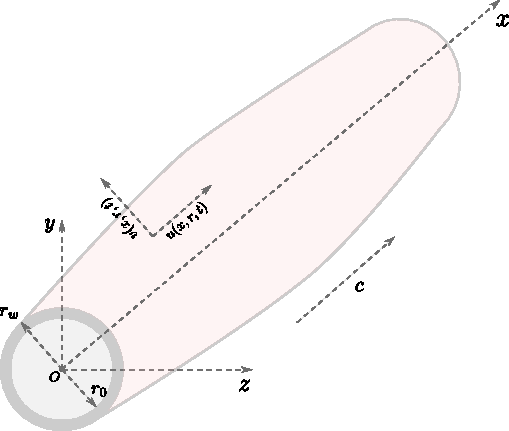
\includegraphics[width=0.55\linewidth]{sketch.pdf}
    \caption{Sketch of a cylindrical elastic vessel subject to an axi-symmetric deformation filled with an ideal fluid.}
    \label{fig:sketch3d}
\end{figure}

\begin{figure}
    \centering
    \begin{subfigure}{0.49\textwidth}
        \centering
        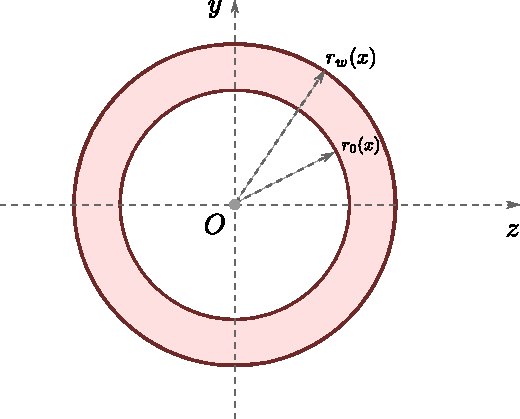
\includegraphics[width=\linewidth]{Axis.pdf}
        \caption{An axi-symmetric deformation.}
        \label{fig:axi}
     \end{subfigure}
     \begin{subfigure}{0.49\textwidth}
        \centering
        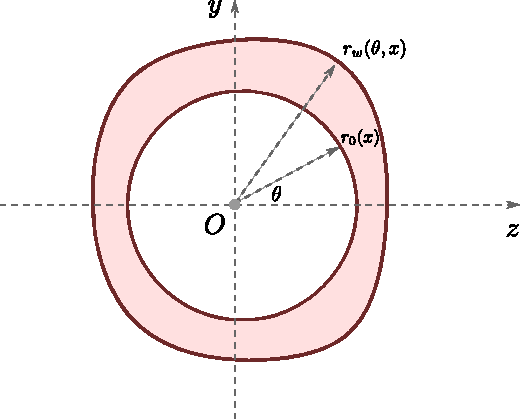
\includegraphics[width=\linewidth]{Gen.pdf}
        \caption{A generic deformation.}
        \label{fig:gen}
    \end{subfigure}
    \caption{A schematic illustration of an axi-symmetric (left panel) and a generic (right panel) deformations of initially cylindrical vessel cross-section. In the sequel, we are going to employ the polar coordinates in the $Oyz$ plane.}
    \label{fig:axisym}
\end{figure}

Finally, we apply the long wave approximation \cite{Dutykh2007, Khakimzyanov2019}. This simplifying assumption can be justified in the following way. Indeed, the Moens--Korteweg celerity $c_{MK} = \O\,(10^2)$ \si{cm \per s} \cite{Tijsseling2012, Lagree2000} and the hear pulsation period is $t_{h} = \O\,(1)$ \si{s}. Consequently, the pulse wavelength can be estimated to be $\lambda = c_{MK}\cdot t_{h} = \O\,(10^2)$ \si{cm}, which is much larger than a typical diameter or arteries approximately equal to $\O\,(1)$ \si{cm}. Henceforth, the long wave assumption can be justified in this way. It is also well-known that long waves are much less affected by the viscosity \cite{Boussinesq1895, Lamb1932, Dutykh2007}, which allows us to adopt the ideal fluid assumption. If necessary, the dissipative effects can be added later along the lines of our previous works on this topic \cite{DutykhDias2007, Dutykh2008a, Dutykh2009c, Mitsotakis2019}. We would like to mention that the long wave approximation is not new \emph{per se}. However, historically, it has been employed to derive hydrostatic models, \emph{cf.} \cite{Lambert1958, Formaggia2003, Quarteroni2004, Delestre2013}. The models resulting from this approach are usually of the hyperbolic type similar to Saint-Venant equations stemming from hydraulics and water pipe flows modelling \cite{Bourdarias2007a, Bourdarias2007, Bourdarias2012}. The peculiarity of our approach is that we go one step further in the hierarchy of models, and we include frequency dispersion effects \cite{Khakimzyanov2016c}.

\subsection{Base model: dimensional formulation}

Taking into account the simplifying assumptions stated above, we can finally formulate our base model in scaled (physical and dimensional) variables by following \cite{Mitsotakis2018, Mitsotakis2019}:
\begin{alignat}{1}
   u_{\,t}\ +\ u\,u_{\,x}\ +\ v\,u_{\,r}\ +\ \frac{1}{\rho}\;p_{\,x}\ &=\ 0\,, \label{eq:momu} \\
   v_{\,t}\ +\ u\,v_{\,x}\ +\ v\,v_{\,r}\ +\ \frac{1}{\rho}\;p_{\,r}\ &=\ 0\,, \label{eq:momv} \\
   r\,u_{\,x}\,+\,(\,r\,v\,)_{\,r}\ &=\ 0\,, \label{eq:inc}
\end{alignat}
where $\rho$ is the constant fluid density, $u$ and $v$ are horizontal and radial particle velocity vector components, respectively, and $p$ is the fluid pressure. The subscripts with independent variables denote the partial derivatives with respect to those variables. We denote by $r^{w}\,(x,t)$ the distance between the cylinder axis and the elastic vessel's wall at a distance $x$ and at time instance $t\ \geq\ 0\,$. The static equilibrium position of the elastic wall is denoted by $r_{0}\,(x)$. See the sketch of the fluid/solid domain in \cref{fig:sketch3d}. The elastic wall radial excursion will be denoted by $\eta\,(x,t)$ and the following relation holds:
\begin{equation*}
    r^{w}\,(x,t) = r_{0}\,(x) + \eta\,(x,t)\,.
\end{equation*}
\cref{eq:momu,eq:momv,eq:inc} should be supplemented with appropriate initial and boundary conditions to obtain a well-posed\footnote{The well-posedness proof for this \gls{ibvp} is left to future works on this subject.} \gls{ibvp}. In order to avoid some obvious singularities, we impose the following condition:
\begin{equation*}
    v\,(x,\,0,\,t)\ =\ 0\,.
\end{equation*}
The elastic wall kinematic impermeability condition reads:
\begin{equation*}
  \eta_{t}\ +\ r^{w}_{x}\cdot u\ =\ v\ \quad\ \mbox{at}\ \quad\ r\ =\ r^{w}\,.
\end{equation*}
The dynamic boundary condition is nothing else but the expression of the forces balance written on vessel walls:
\begin{equation*}
    \rho^{w}\,h\,\eta_{tt}\ =\ p^{w}\ -\ \frac{E\,h}{r_{\,0}^{\,2}\,(1\,-\,\nu^2)}\:\eta\ \quad\ \mbox{at}\ \quad\ r\ =\ r^{w}\,,
\end{equation*}
where $\rho^{w}$ is the wall density, $p^{w}$ is the pressure exerted by the fluid on the elastic wall, $h$ is the wall thickness, $E$ and $\nu$ characterize the elastic properties (Young modulus and Poisson ratio correspondingly) of the vessel. In this study, we assume for simplicity that $E$, $\nu$, $\rho^{w}$, and $h$ are constants.

\subsection{Potential model: dimensional formulation}

We next recast the governing equations in terms of a velocity potential. Assuming the flow to be incompressible, irrotational, and axisymmetric, we introduce a smooth potential
\[
  \phi\ =\ \phi(x,r,t),\qquad
  (u,v)^{\top}\ =\ \nabla\phi\ =\ (\phi_{x},\phi_{r})^{\top},
\]
so that the Euler equations reduce to the Cauchy--Lagrange integral on the moving wall \cite{Mitsotakis2019}:
\begin{equation}\label{eq:bernouli}
  \phi_{t}
  +\tfrac{1}{2}\,\phi_{x}^{2}
  +\tfrac{1}{2}\,\phi_{r}^{2}
  +\frac{1}{\rho}\,p
  +\kappa\,\phi
  \;=\;0,
  \qquad
  r=r^{w}.
\end{equation}
Here the instantaneous wall position is
\(
  r^{w}=r_{0}(x)+\eta(x,t),
\)
with $r_{0}$ the unperturbed radius and $\eta$ the wall displacement. Under the potential-flow assumption the continuity equation becomes
\begin{equation}\label{eq:massp}
  r\,\phi_{xx}\ +\ \bigl(r\,\phi_{r}\bigr)_{r}\ =\ 0, \qquad 0\ <\ r\ <\ r^{w}\,,
\end{equation}
while the kinematic boundary conditions read
\begin{align}
  \phi_{r}&=0,
  & r&=0, \label{eq:bc1p}\\[2pt]
  \phi_{r}&=\eta_{t}+r^{w}_{x}\,\phi_{x},
  & r&=r^{w}(x,t).\label{eq:bc2p}
\end{align}
Equations \eqref{eq:bernouli}--\eqref{eq:bc2p} furnish the starting point for the long-wave asymptotics carried out in the sequel of this study.

\subsubsection{Variational principles}
\label{sec:var_principles}

Two complementary variational frameworks are commonly employed for irrotational surface-wave problems: Luke's Lagrangian formulation \cite{Luke1967} and the Hamiltonian formulation of Petrov and Zakharov \cite{Petrov1964, Zakharov1968}. Surveys by \cite{Radder1999} and \cite{Zakharov1997} provide extensive historical background. Luke's principle incorporates the velocity potential directly and imposes irrotationality \emph{a priori}, whereas Zakharov's Hamiltonian requires both incompressibility and bottom impermeability to be satisfied identically, thereby rendering it more restrictive. In either case the free‐surface conditions arise from the stationarity of an action functional in which part of the bulk dynamics is built in exactly and the remainder is obtained by variation. The earliest use of a pressure‐based Lagrangian is due to \cite{Clebsch1859} and \cite{Hargreaves1908}, although the concomitant free‐surface boundary conditions were not explicitly recognised at the time. The following derivation highlights this connection. Recently, the variational techniques have been successfully applied to model water waves in various asymptotic regimes \cite{Clamond2009,Clamond2024}.

\paragraph{Lagrangian formulation.} First, for the irrotational case, let $\phi\,(x,\,r,\,t\,)$ be the velocity potential of a fluid lying between $r\,=\,0$ and $r\,=\,r^{\,w}\,(\,x,\,t\,)\,$. The variational principle (\cite{Luke1967}) is given by
\begin{equation}\label{eq:chap5.1}
  \delta J\,=\,\delta\,\int_{\,t_{1}}^{\,t_{2}}\,\int_{\,x_{\,1}}^{\,x_{\,2}}\,\mathcal{L}\,\mathrm{d}x\,\mathrm{d}t\,=\,0\,,\quad \text{with} \quad \mathcal{L}\,=\,\int_{\,0}^{\,r^{\,w}}\,\biggl(\phi_{\,t} \,+\,\frac{1}{2}\;\phi_{\,x}^{\,2} \,+\,\frac{1}{2}\;\phi_{\,r}^{\,2}\,\biggr)\,r\,\mathrm{d}r\,-\,\frac{1}{2}\;\alpha\,\eta_{\,t}^{\,2} \,-\,\frac{1}{2}\,\beta\,\eta^{\,2}\,+\,p^{\,w}\,\eta\,,
\end{equation}
where $\phi\,(\,x,\,r,\,t\,)$ and $r^{\,w}\,(\,x,\,t\,)$ are allowed to vary subject to the restrictions $\delta\,\phi\,=\,0$ and $\delta \,r^{\,w}\,=\,0$ at $x_{\,1},\,x_{\,2},\,t_{\,1}$ and $t_{\,2}$. The only difference from classical formulations using pressure expressions is that $r^{\,w}\,(\,x,\,t\,)$ variations are permitted here. Following standard procedures from the calculus of variations, equation \eqref{eq:chap5.1} becomes
\begin{multline}
  \delta J\,=\,\int_{\,t_{\,1}}^{\,t_{\,2}}\,\int_{\,x_{\,1}}^{\,x_{\,2}}\,\Biggl[\biggl(\,\phi_{\,t}\,+\,\frac{1}{2}\;\phi_{\,x}^{\,2}\,+\,\frac{1}{2}\;\phi_{\,r}^{\,2}\,\biggr)\,r\,\Biggr]_{\,r\,=\,r^{\,w}}\,\delta r^{\,w}
  \\[0.5em]
  +\,\int_{\,0}^{\,r^{\,w}}\,\bigl(\,\phi_{\,x}\,\delta \phi_{\,x}\,+\,\phi_{\,r}\,\delta \phi_{\,r}\,+\,\delta \phi_{\,t}\,\bigr)\,r\,\mathrm{d}r\,\Biggr]\,\mathrm{d}x\,\mathrm{d}t
  \\[0.5em]
  +\,\delta\,\int_{\,t_{\,1}}^{\,t_{\,2}}\,\int_{\,x_{\,1}}^{\,x_{\,2}}\,\biggl(\,\frac{1}{2}\;\alpha\,\eta_{\,t}^{\,2} \,-\,\frac{1}{2}\;\beta\,\eta^{\,2} \,-\,p^{\,w}\,\eta\,\biggr)\,\mathrm{d}x\,\mathrm{d}t\,=\,0\,.
\end{multline}
Natural boundary conditions at $r\,=\,0$ and $r\,=\,r^{\,w}$ follow from the careful integration of \eqref{eq:chap5.1}. We consider the decomposition:
\begin{enumerate}
\item $\int_{\,0}^{\,r^{\,w}}\,r\,\phi_{\,x}\,\delta \phi_{\,x}\,\mathrm{d}r\,=\,\int_{\,0}^{\,r^{\,w}}\,\bigl[\,r\,\phi_{\,x}\,\delta \phi\,\bigr]_{\,x}\,\mathrm{d}r\,-\,\int_{\,0}^{\,r^{\,w}}\,r\,\phi_{\,xx}\,\delta \phi\,\mathrm{d}r =\,-\,r_{\,x}^{\,w}\,r^{\,w}\,\phi_{\,x}\,\delta \phi\,\biggr|_{\,r\,=\,r^{\,w}}\,+\,\partial_{\,x}\,\int_{\,0}^{\,r^{\,w}}\,r\,\phi_{\,x}\,\delta \phi\,\mathrm{d}r\,,$
\item $\int_{\,0}^{\,r^{\,w}}\,r\,\phi_{\,r}\,\delta \phi_{\,r}\,\mathrm{d}r\,=\,\bigl[\,r\,\phi_{\,r}\,\delta \phi\,\bigr]_{\,r\,=\,0}^{\,r\,=\,r^{\,w}}\,-\,\int_{\,0}^{\,r^{\,w}}\,\bigl(\,\phi_{\,r}\,+\,r\,\phi_{\,rr}\,\bigr)\,\delta \phi\,\mathrm{d}r\,,$
\item $\int_{\,0}^{\,r^{\,w}}\,r\,\delta \phi_{\,t}\,\mathrm{d}r\,=\,\int_{\,0}^{\,r^{\,w}}\,\partial_{\,t}\,(r\,\delta \phi)\,\mathrm{d}r\,=\,-\,r^{\,w}\,r_{\,t}\,\delta \phi\,\biggr|_{\,r\,=\,r^{\,w}}\,+\,\partial_{\,t}\,\int_{\,0}^{\,r^{\,w}}\,r\,\delta \phi\,\mathrm{d}r\,.$
\end{enumerate}
Additionally, we compute
\begin{equation*}
  \delta\,\int_{\,t_{\,1}}^{\,t_{\,2}}\,\int_{\,x_{\,1}}^{\,x_{\,2}}\,\biggl(\,-\,\frac{1}{2}\;\alpha\,\eta_{\,t}^{\,2}\,-\,\frac{1}{2}\;\beta\,\eta^{\,2}\,+\,p^{\,w}\,\eta\,\biggr)\,\mathrm{d}x\,\mathrm{d}t\,=\,\int_{\,t_{\,1}}^{\,t_{\,2}}\,\int_{\,x_{\,1}}^{\,x_{\,2}}\,\bigl(\,-\,\alpha\,\eta_{\,t}\,\delta \eta_{\,t}\,-\,\beta\,\eta\,\delta \eta\,+\,p^{\,w}\,\delta \eta\,\bigr)\,\mathrm{d}x\,\mathrm{d}t\,.
\end{equation*}
Substituting all these contributions into \eqref{eq:chap5.1}, we obtain
\begin{multline*}
  \delta J\,=\,\int_{\,t_{\,1}}^{\,t_{\,2}}\,\int_{\,x_{\,1}}^{\,x_{\,2}}\,\Biggl[\biggl(\,\phi_{\,t}\,+\,\frac{1}{2}\;\phi_{\,x}^{\,2}\,+\,\frac{1}{2}\;\phi_{\,r}^{\,2}\,\biggr)\,r\,\Biggr]_{\,r\,=\,r^{\,w}}\,\delta r^{\,w} \\
  -\,\bigl[\,r\,\phi_{\,r}\,\delta \phi\,\bigr]_{\,r\,=\,0} \,-\,\int_{\,0}^{\,r^{\,w}}\,\bigl(\,r\,\phi_{\,xx}\,+\,\phi_{\,r}\,+\,r\,\phi_{\,rr}\,\bigr)\,\delta \phi\,\mathrm{d}r\,\Biggr]\,\mathrm{d}x\,\mathrm{d}t \\
  +\,\int_{\,t_{\,1}}^{\,t_{\,2}}\,\int_{\,x_{\,1}}^{\,x_{\,2}}\,\bigl(\,-\,\alpha\,\eta_{\,tt}\,-\,\beta\,\eta\,+\,p^{\,w}\,\bigr)\,\delta \eta\,\mathrm{d}x\,\mathrm{d}t\,=\,0\,.
\end{multline*}
Taking $\delta r^{\,w}\,=\,0$ and assuming $\delta \phi\big|_{\,r\,=\,r^{\,w}}\,=\,\delta \phi\big|_{\,r\,=\,0}\,=\,0\,$, and noting that $\delta \phi$ is otherwise arbitrary, we deduce the following system:
\begin{align}
  \phi_{\,t}\,+\,\frac{1}{2}\;\phi_{\,x}^{\,2}\,+\,\frac{1}{2}\;\phi_{\,r}^{\,2}\,-\,\alpha\,\eta_{\,tt}\,-\,\beta\,\eta\,+\,p^{\,w} &=\,0 \,, & r\,=\,r^{\,w}\,(x,\,t)\,, \label{eq:chap5.2}\\[0.5em]
  r\,\phi_{\,xx}\,+\,(\,r\,\phi_{\,r}\,)_{\,r} &=\,0 \,, & 0\,<\,r\,<\,r^{\,w}\,(x,\,t)\,, \label{eq:chap5.3}\\[0.5em]
  \phi_{\,r} &=\,0\,, & r\,=\,0\,, \label{eq:chap5.4}\\[0.5em]
  \phi_{\,r} &=\,\eta_{\,t}\,+\,r^{\,w}_{\,x}\,\phi_{\,x}\,, & r\,=\,r^{\,w}\,(x,\,t)\,, \label{eq:chap5.5}\\[0.5em]
  p^{w} &=\,\alpha\,\eta_{\,tt}\,+\,\beta\,\eta\,, & r\,=\,r^{\,w}\,(x,\,t)\,. \label{eq:chap5.6}
\end{align}

Thus, we observe that the variational principle \eqref{eq:chap5.1} elegantly recovers the complete potential flow formulation for our problem. Equation \eqref{eq:chap5.3} represents the Laplace equation in cylindrical coordinates, which governs the irrotational flow in the fluid domain. The boundary conditions are given by the impermeability condition at the axis of symmetry \eqref{eq:chap5.4} and the kinematic condition at the vessel wall \eqref{eq:chap5.5}. The dynamic condition \eqref{eq:chap5.2} corresponds to the Cauchy--Lagrange integral at the vessel wall, while \eqref{eq:chap5.6} describes the pressure law for the viscoelastic wall. This demonstrates the power of variational methods in deriving the governing equations for fluid-structure interaction problems in a systematic and physically consistent manner.

\paragraph{Hamiltonian formulation.}

This section belongs to the relatively recent trend of applying concepts from Hamiltonian mechanics to problems in fluid dynamics. By 'Hamiltonian mechanics', we refer to the entirety of classical mechanics in the spirit of foundational texts such as \cite{Lanczos1970, Goldstein2001,Arnold1997}, encompassing both particle mechanics and field theory. Hamiltonian approaches have proven indispensable in classical and quantum theories of particles and fields. If their only contribution were a reformulation of known results, they would be of limited value. However, substantial evidence indicates that classical mechanics methods offer a powerful and unifying framework in fluid dynamics as well. Several factors account for the effectiveness of Hamiltonian approaches. Firstly, Hamilton's formalism provides an elegant and economical representation of dynamics. Secondly, the well-established connection between symmetries of the Hamiltonian and conservation laws facilitates the construction of approximate models that preserve analogues of exact invariants. Thirdly, Hamiltonian formulations are coordinate-invariant and thus adaptable to diverse geometrical settings. In Hamiltonian perturbation theory, for instance, dynamical approximations are naturally associated with transformations of the dependent variables. This flexibility enables one to simultaneously adjust the physical description and its mathematical representation to obtain models in their simplest possible form.

We now consider the motion governed by equations \eqref{eq:chap5.2}–\eqref{eq:chap5.6}. The total energy of the system comprises the kinetic energy, potential energy, and surface energy, and is normalised such that the total energy vanishes in the quiescent state. The evolution equations take the abstract Hamiltonian form
\begin{equation}
  \begin{pmatrix}
    \eta_{\,t} \\
    \psi_{\,t}
  \end{pmatrix}
  \,=\,\mathcal{J}
  \begin{pmatrix}
    \displaystyle\frac{\delta\mathcal{H}}{\delta\,\eta} \\[0.8em]
    \displaystyle\frac{\delta\mathcal{H}}{\delta\,\psi}
  \end{pmatrix},
  \qquad
  \mathcal{J}\,=\,\begin{pmatrix}
    0 & \mathbb{I} \\
    -\mathbb{I} & 0
  \end{pmatrix},
\end{equation}
where $\delta\mathcal{H}$ denotes the Gâteaux (variational) derivative, $\psi\,\equiv\,\phi\,(\,x,\,r,\,t\,)|_{\,r\,=\,r^{\,w}\,(\,x,\,t\,)}$ is the surface potential, and the Hamiltonian density and total energy are given by
\begin{equation}
  H\,=\,\frac{1}{2}\,\int_{0}^{\eta}\,|\,\nabla\phi\,|^{\,2}\,\mathrm{d}r\,+\,\biggl(\,-\,\frac{1}{2}\,\alpha\,\eta_{\,t}^{\,2}\,-\,\frac{1}{2}\,\beta\,\eta^{\,2}\,+\,p^{\,w}\,\eta\,\biggr), \qquad
  \mathcal{H}\,=\,\int_{\mathbb{R}}\,H\,\mathrm{d}x\,.
\end{equation}
We now compute the variation of the Hamiltonian functional under the perturbation $\eta \mapsto \eta + \delta \eta$:
\begin{multline*}
  \mathcal{H}\,[\,\eta\,+\,\delta\eta,\,\phi\,]\,-\,\mathcal{H}\,[\,\eta,\,\phi\,]
  \,=\,\frac{1}{2}\,\int_{\mathbb{R}}\,\int_{0}^{\eta+\delta\eta}\,|\,\nabla\phi\,|^{\,2}\,\mathrm{d}r\,\mathrm{d}x
  \\[0.5em]
  -\,\frac{1}{2}\,\alpha\,\int_{\mathbb{R}}\,(\,\eta\,+\,\delta\eta\,)_{\,t}^{\,2}\,\mathrm{d}x
  -\,\frac{1}{2}\,\beta\,\int_{\mathbb{R}}\,(\,\eta\,+\,\delta\eta\,)^{\,2}\,\mathrm{d}x
  +\,\int_{\mathbb{R}}\,p^{\,w}\,(\,\eta\,+\,\delta\eta\,)\,\mathrm{d}x
  \\[0.5em]
  -\,\frac{1}{2}\,\int_{\mathbb{R}}\,\int_{0}^{\eta}\,|\,\nabla\phi\,|^{\,2}\,\mathrm{d}r\,\mathrm{d}x
  +\,\frac{1}{2}\,\alpha\,\int_{\mathbb{R}}\,\eta_{\,t}^{\,2}\,\mathrm{d}x
  +\,\frac{1}{2}\,\beta\,\int_{\mathbb{R}}\,\eta^{\,2}\,\mathrm{d}x
  -\,\int_{\mathbb{R}}\,p^{\,w}\,\eta\,\mathrm{d}x\,.
\end{multline*}
After simplification, we obtain
\begin{equation*}
  \mathcal{H}\,[\,\eta\,+\,\delta\eta,\,\phi\,]\,-\,\mathcal{H}\,[\,\eta,\,\phi\,]
  \,=\,\frac{1}{2}\,\int_{\mathbb{R}}\,\int_{\eta}^{\eta+\delta\eta}\,|\,\nabla\phi\,|^{\,2}\,\mathrm{d}r\,\mathrm{d}x\,-\,\alpha\,\int_{\mathbb{R}}\,\eta_{\,t}\,\delta\eta_{\,t}\,\mathrm{d}x\,-\,\beta\,\int_{\mathbb{R}}\,\eta\,\delta\eta\,\mathrm{d}x
  +\,\int_{\mathbb{R}}\,p^{\,w}\,\delta\eta\,\mathrm{d}x\,.
\end{equation*}
Applying the mean value theorem to the integral over the interval $[\eta,\,\eta+\delta\eta]$, we finally obtain
\begin{equation*}
  \mathcal{H}\,[\,\eta\,+\,\delta\eta,\,\phi\,]\,-\,\mathcal{H}\,[\,\eta,\,\phi\,]
  \,=\,\frac{1}{2}\,\int_{\mathbb{R}}\,\bigl[\,|\,\nabla\phi\,|^{\,2}\,\bigr]_{\,r\,=\,r^{\,w}}\,\delta\eta\,\mathrm{d}x\,-\,\alpha\,\int_{\mathbb{R}}\,\eta_{\,tt}\,\delta\eta\,\mathrm{d}x
  -\,\beta\,\int_{\mathbb{R}}\,\eta\,\delta\eta\,\mathrm{d}x
  +\,\int_{\mathbb{R}}\,p^{\,w}\,\delta\eta\,\mathrm{d}x\,.
\end{equation*}
Therefore, the non-canonical Hamiltonian evolution equations take the form
\begin{equation}
  \begin{pmatrix}
    \eta_{\,t} \\
    \psi_{\,t}
  \end{pmatrix}
  \,=\,\begin{pmatrix}
    \phi_{\,r}\,-\,r^{\,w}_{\,x}\,\phi_{\,x} \\
    -\,\frac{1}{2}\,|\,\nabla\phi\,|^{\,2}\,+\,\alpha\,\eta_{\,tt}\,+\,\beta\,\eta\,-\,p^{\,w}
  \end{pmatrix},
\end{equation}
which recover the dynamic and kinematic boundary conditions \eqref{eq:chap5.2} and \eqref{eq:chap5.5}, respectively. It is important to emphasise that the operator $\mathcal{J}$ is skew-symmetric and satisfies the Jacobi identity (cf. \cite{Nutku1987}), thus qualifying as a legitimate Hamiltonian operator.

In conclusion, the derivation and analysis of the non-canonical Hamiltonian structure provide a robust and systematic framework for investigating complex dynamical systems governed by nonlinear wave equations. The geometric properties of the Hamiltonian operator, including skew-symmetry and the Jacobi identity, ensure consistency with the underlying physics. This insight not only strengthens the theoretical foundations but also enhances the practical modelling of nonlinear dispersive systems in mathematical physics.

\subsection{Potential model: dimensionless formulation and the first derivation of the long wave model}\label{sec:dimless_longwave}

To develop an asymptotic reduction of the Euler system we introduce the non-dimensional variables
\begin{equation}\label{eq:ndv}
  \eta^{\ast}=\frac{\eta}{a},\quad
  x^{\ast}=\frac{x}{\lambda},\quad
  r^{\ast}=\frac{r}{R},\quad
  t^{\ast}=\frac{t}{T},\quad
  \phi^{\ast}=\frac{\phi}{\lambda\,\varepsilon\,\tilde{c}},\quad
  p^{\ast}=\frac{p}{\varepsilon\,\rho\,\tilde{c}^{2}},
\end{equation}
where $a$ is the typical wall displacement, $\lambda$ a characteristic wavelength, $R$ the mean radius, and $T=\lambda/\tilde{c}$ the advective time scale with
\(
  \tilde{c}=\sqrt{E h/(2\rho R)}
\)
the Moens--Korteweg speed \cite{Fung2013}. The small parameters
\begin{equation}\label{eq:eps_del}
  \varepsilon\ \eqdef\ \frac{a}{R}, \qquad \delta\ \eqdef\ \frac{R}{\lambda},
\end{equation}
measure nonlinearity and dispersion, respectively; throughout we assume $\varepsilon = \O(1)$ and $\delta^{2}\ \ll\ 1$. Dropping the asterisks henceforth, the dimensionless system becomes
\begin{align}
  & \phi_{t}
    +\tfrac{\varepsilon}{2}\,\phi_{x}^{2}
    +\tfrac{\varepsilon}{2\delta^{2}}\,
     \phi_{r}^{2}
    +p
    +\varepsilon\kappa\,\phi
    =0,
    && r=r^{w}, \label{eq1}\\[2pt]
  & \delta^{2}\,r\,\phi_{xx}
    +\bigl(r\,\phi_{r}\bigr)_{r}
    =0,
    && 0<r<r^{w}, \label{eq2}\\[2pt]
  & \phi_{r}=0,
    && r=0, \label{eq3}\\[2pt]
  & \phi_{r}
    =\delta^{2}\eta_{t}
     +\delta^{2}\bigl(r_{0}(x)+\varepsilon\eta\bigr)_{x}\,\phi_{x},
    && r=r^{w}, \label{eq4}\\[2pt]
  & p
    =\alpha\,\delta^{2}\,\eta_{tt}
     +\beta\bigl(\eta+\delta^{2}\gamma\,\eta_{t}\bigr),
    && r=r^{w}, \label{eq5}
\end{align}
where
\(
  \kappa\ =\ \kappa^{\ast},\;
  \alpha\ =\ \rho^{w}h/(\rho R),\;
  \beta\ =\ \beta(x)\ =\ 2R^{2}/r_{0}^{2}(x),\;
  \gamma\ =\ \gamma^{\ast}
\)
(cf.\,\cite{Mitsotakis2019}).

\paragraph{Asymptotic expansion of the velocity potential.} Following \cite{BCS}, we expand
\begin{equation}\label{eq:potential}
  \phi(x,r,t)\;=\;\sum_{m=0}^{\infty} r^{m}\,\phi_{m}(x,t).
\end{equation}
Insertion into \eqref{eq2} yields the recursion
\begin{equation}\label{eq:recurr}
  \delta^{2}\partial_{x}^{2}\phi_{2m}
  +(2m+2)^{2}\phi_{2m+2}=0,
  \qquad
  \phi_{2m+1}=0,
  \quad m\ \in\ \{0,1,2,\dots\}.
\end{equation}
so that
\begin{equation}\label{eq:phi2}
  \phi_{2}=-\frac{\delta^{2}}{4}\,\partial_{x}^{2}\phi_{0},
\end{equation}
and, for $m\ge1$,
\begin{equation}\label{eq:phim}
  \phi_{2m+2}
  =\frac{\delta^{4}}{(2m+2)^{2}(2m)^{2}}\,
   \partial_{x}^{4}\phi_{2m-2}
  =\O(\delta^{4}).
\end{equation}
Retaining terms up to $O(\delta^{4})$ gives
\begin{equation}\label{eq:potapr}
  \phi(x,r,t)
  \;=\;
  \phi_{0}(x,t)
  -\delta^{2}\frac{r^{2}}{4}\,\partial_{x}^{2}\phi_{0}
  +\delta^{4}\frac{r^{4}}{64}\,\partial_{x}^{4}\phi_{0}
  +\O(\delta^{6}).
\end{equation}

\paragraph{Kinematic boundary condition.} Using \eqref{eq:potapr} in \eqref{eq4} we obtain, to $O(\delta^{4})$,
\begin{equation}\label{eq:massp1}
  \eta_{t}
  +r^{w}_{x}\,\phi_{0\,x}
  +\frac{r^{w}}{2}\,\phi_{0\,xx}
  -\delta^{2}\frac{(r^{w})^{2}r^{w}_{x}}{4}\,\phi_{0\,xxx}
  -\delta^{2}\frac{(r^{w})^{3}}{16}\,\phi_{0\,xxxx}
  =\O(\delta^{4}).
\end{equation}

\paragraph{Dynamic boundary condition.} Combining \eqref{eq1} with \eqref{eq5} eliminates the pressure and, after substitution of \eqref{eq:potapr}, yields
\begin{align}\label{eq:momentump1}
  \phi_{0\,t}
  &-\delta^{2}\frac{(r^{w})^{2}}{4}\,\phi_{0\,xxt}
   +\frac{\varepsilon}{2}\Bigl(
       \phi_{0\,x}^{2}
       -\delta^{2}\frac{(r^{w})^{2}}{2}\,\phi_{0\,x}\phi_{0\,xxx}
   \Bigr)
   +\frac{\varepsilon\delta^{2}}{8}(r^{w})^{2}\,\phi_{0\,xx}^{2}
   \notag\\
  &+\varepsilon\kappa
     \Bigl(\phi_{0}
           -\delta^{2}\frac{(r^{w})^{2}}{4}\,\phi_{0\,xx}\Bigr)
   +\alpha\delta^{2}\eta_{tt}
   +\beta\bigl(\eta+\delta^{2}\gamma\,\eta_{t}\bigr)
   = \O(\delta^{4}).
\end{align}

\paragraph{Centreline velocity formulation.} Define
\[
  w(x,t)\coloneqq\phi_{0\,x}(x,t) \equiv u(x,0,t).
\]
Equations \eqref{eq:massp1} and \eqref{eq:momentump1} become
\begin{align}
  &\eta_{t}
   +r^{w}_{x}\,w
   +\frac{r^{w}}{2}\,w_{x}
   -\delta^{2}\frac{(r^{w})^{2}r^{w}_{x}}{4}\,w_{xx}
   -\delta^{2}\frac{(r^{w})^{3}}{16}\,w_{xxx}
   =\O(\delta^{4}),\label{eq:massp2}\\
  &w_{t}+(\beta\eta)_{x}
   +\varepsilon w\,w_{x}
   -\frac{\delta^{2}}{4}\bigl[(r^{w})^{2}\Gamma\bigr]_{x}
   +\varepsilon\kappa
      \Bigl[w-\frac{\delta^{2}}{4}\bigl((r^{w})^{2}w_{x}\bigr)_{x}\Bigr]
   +\alpha\delta^{2}\eta_{x t t}
   +\delta^{2}\gamma(\beta\eta_{t})_{x}
   = \O(\delta^{4}),\label{eq:momentump2}
\end{align}
with
\begin{equation}\label{eq:gamma}
  \Gamma=w_{x t}
         +\varepsilon w\,w_{xx}
         -\frac{\varepsilon}{2}\,w_{x}^{2}.
\end{equation}
These equations \eqref{eq:massp2}--\eqref{eq:gamma} constitute the celebrated Serre--Green--Naghdi system of fully nonlinear weakly dispersive equations. This system will be rederived below without the irrotational flow assumption, providing a more general framework for our analysis.

\subsubsection{Enhanced Serre-type system}\label{sec:cbsys}

To improve the model we evaluate the horizontal velocity at an arbitrary radius $r\ =\ \theta\,r^{w}$ ($0 \leq \theta \leq 1$). From \eqref{eq:potapr}
\[
  u(x,r,t)
  =w
   -\delta^{2}\frac{r^{2}}{4}\,w_{xx}
   +\O(\delta^{4}),
  \qquad
  u^{\theta}(x,t) \ \eqdef\ u(x,\theta r^{w},t)
  =w-\delta^{2}\theta^{2}\frac{(r^{w})^{2}}{4}\,w_{xx}+\O(\delta^{4}),
\]
so that
\begin{equation}\label{eq:generalu}
  w=u^{\theta}
    +\delta^{2}\theta^{2}\frac{(r^{w})^{2}}{4}\,u^{\theta}_{xx}
    +\O(\delta^{4}).
\end{equation}
Substituting \eqref{eq:generalu} into \eqref{eq:massp2} gives
\begin{equation}\label{eq:massp4}
  \eta_{t}
  +r^{w}_{x}\,u^{\theta}
  +\frac{r^{w}}{2}\,u^{\theta}_{x}
  +\delta^{2}\frac{(2\theta^{2}-1)(r^{w})^{2}r^{w}_{x}}{4}\,
        u^{\theta}_{xx}
  +\delta^{2}\frac{(2\theta^{2}-1)(r^{w})^{3}}{16}\,
        u^{\theta}_{xxx}
  =O(\delta^{4}).
\end{equation}
Using $r^{w}_{t}=\varepsilon\eta_{t}$ together with
\eqref{eq:generalu} in \eqref{eq:momentump2} yields
\begin{equation}\label{eq:momentump4}
  u^{\theta}_{t}
  +(\beta\eta)_{x}
  +\varepsilon u^{\theta}u^{\theta}_{x}
  +\frac{\delta^{2}}{4}
     \Bigl\{\theta^{2}(r^{w})^{2}\Gamma_{x}
            -\bigl[(r^{w})^{2}\Gamma\bigr]_{x}\Bigr\}
  +\varepsilon\kappa\,Q
  +R
  = \O(\delta^{4}),
\end{equation}
where
\begin{equation}\label{eq:gamman}
  \Gamma
  =u^{\theta}_{x t}
   +\varepsilon u^{\theta}u^{\theta}_{xx}
   -\frac{\varepsilon}{2}(u^{\theta}_{x})^{2},\quad
  Q
  =u^{\theta}
   +\frac{\delta^{2}}{4}(\theta^{2}-1)(r^{w})^{2}u^{\theta}_{xx}
   -\delta^{2}r^{w}r^{w}_{x}u^{\theta}_{x},\quad
  R
  =\alpha\delta^{2}\eta_{x t t}
   +\delta^{2}\gamma(\beta\eta_{t})_{x}.
\end{equation}
The choice $\theta^{2}\ =\ 1/2$ recovers the classical Serre-type approximation.

\subsection{Base model: dimensionless formulation}

In this Section, we elaborate on the scaled formulation for the Euler equations in cylindrical coordinates presented above. The first step consists of introducing non-dimensional independent variables, which are defined as follows:
\begin{equation*}
  \eta^{\,\star}\,=\;\frac{\eta}{\,a}\;,\quad x^{\,\star}\,=\;\frac{x}{\,\lambda}\;,\quad r^{\,\star}\,=\;\frac{r}{R}\;,\quad t^{\,\star}\,=\;\frac{t}{T}\;,\quad u^{\,\star}\,=\;\frac{1}{\eps\, \tilde{\,c}}\;u, \quad v^{\,\star}\,=\;\frac{1}{\eps\,\delta\,\tilde{c}}\;v, \quad p^{\,\star}\,=\;\frac{1}{\eps\,\rho\, \tilde{c}^{\,2}}\;p\,,
\end{equation*}
where $a$ is a typical amplitude of the vessel wall displacement, $\lambda$ a typical wavelength of a pulse, $R$ is a vessel's typical radius, $ t\,=\,\lambda$\,/\,\,$\tilde{c}\,$ the characteristic timescale, while $\tilde{c}\,=\,\sqrt{E\,h\,/\,2\, \rho\,R}$ is the Moens-Korteweg characteristic speed \cite{Fung1997a}. The parameters $\eps$ and $\delta$ characterize the non-linearity and the non-hydrostatic effects in the system:
\begin{equation*}
  \eps\,\coloneqq\, \frac{a}{R}\;, \quad \delta\,\coloneqq\,\frac{R}{\lambda}\;.
\end{equation*}
In the present work, we aim to keep $\eps = \O(1)$ as long as possible while assuming from the outset that $\delta^2 \ll 1$ is a small parameter.

Omitting the $\star$ symbol from the notation below for the sake of simplicity, the non-dimensional form of the Euler takes the form (holding for $0\, < \,r\, <\, r^{\,w}\,\coloneqq\,r_{\,0}\,+\,\eps\,\eta$) \cite{Mitsotakis2018}:
\begin{equation}\label{eq:momentx}
  u_{\,t}\,+\,\eps\,u\,u_{\,x}\,+\,\eps\,v\, u_{\,r}\,+\,p_{\,x}\ =\ 0\,,
\end{equation}
\begin{equation}\label{eq:momenty}
  \delta^{\,2}\,(\,v_{\,t}\,+\,\eps\,u\,v_{\,x}\,+\,\eps\,v \,v_{\,r}\,)\,+\,p_{\,r}\ =\ 0\,,
\end{equation}
\begin{equation}\label{eq:cont}
  r\,u_{\,x}\,+\,(\,r\,v\,)_{\,r}\ =\ 0\,.
\end{equation}
We also add the dimensionless flow irrotationality condition that will be needed in our developments below \cite{Landau1987}:
\begin{equation}\label{eq:irr}
  \delta^{\,2}\,v_{\,x}\ =\ u_{\,r}\,.
\end{equation}
The scaled version of the kinematic boundary condition reads
\begin{equation}\label{eq:kin}
  v\,(\,x\,,\,r^{\,w},\,t\,)\ =\ \eta_{\;t}\,(\,x,\,t\,)\,+\,r_{\,x}^{\,w}\,u\,(\,x,\,r^{\,w},\,t\,)\,,
\end{equation}
while the dynamic boundary condition reads
\begin{equation}\label{eq:dyn}
  p^{\,w}\,(\,x,\,t\,)\,=\,p\,(\,x,\,r^{\,w},\,t\,)\ =\ \alpha\,\delta^{\,2}\,\eta_{\;tt}\,(\,x,\,t\,)\,+\,\beta\,(\,x\,)\,\eta\,(\,x,\,t\,)\,+\,\delta^{\,2}\beta\,\gamma\,\eta_{\;t}\,.
\end{equation}
The non-singularity condition along the symmetry axis reads:
\begin{equation}\label{eq:zero}
  v\,(\,x,\,0,\,t\,)\ =\ 0\,.
\end{equation}
Above, we introduced the following notations:
\begin{equation*}
  \tilde{\alpha}\,\coloneqq\;\frac{\rho^{\,w}\,h}{\rho}\; \quad \text{and} \ \quad \tilde{\beta}(\,x\,)\,\coloneqq\, \frac{E\,h}{\rho\,r_{\,0}^{\,2}\,(\,x\,)}\;. 
\end{equation*}
Then,
\begin{equation*}
  \alpha\,\coloneqq\,\frac{\tilde{\alpha}}{\,R}\;, \quad  \ \quad  \beta\,(\,x\,)\,\coloneqq\,\frac{2\,R^{\,2}\,\rho}{E\,h}\,\tilde{\beta}\,(\,x\,) \quad \text{and} \ \quad \gamma\,\coloneqq\,\tilde{\frac{\gamma }{\delta^{\,2}\,T}\;}\,,
\end{equation*}
where $\rho^{\,w}$ is the wall density, $h$ is the thickness of the vessel wall, $E$ is the young modulus of elasticity, $R$ is a vessel's radius, $T\, \coloneqq \;\displaystyle\frac{\lambda}{c}$ is the characteristic timescale. Below, we use the scaled governing equations in order to propose a simplified model.

\subsection{Derivation of a new fully nonlinear weakly dispersive model}

In this Section, we perform the dimensionality reduction of the axi-symmetric Euler system presented above. In order to achieve this goal, we use essentially two mathematical tools: depth averaging and asymptotic expansions. In the derivation below, we follow the footsteps of our previous works on this topic \cite{Dutykh2011a, Clamond2015c, Khakimzyanov2019, Clamond2024}.

The horizontal velocity is approximated by its depth-averaged value:
\begin{equation}\label{eq:avg}
  \bar{u}(x,t)\ \coloneqq\ \frac{1}{r_{\,0}\;+\,\eps\,\eta}\;\displaystyle \int_{\,0}^{\,r^{\,w}}\,u\,(\,x,\,r,\,t\,)\,\ud\,r\,.
\end{equation}
We start the derivation by integrating the continuity \cref{eq:cont}:
\begin{equation*}
  \int_{\,0}^{\,r^{\,w}}\,r\,u_{\,x}\,\ud\,r \,+\, \int_{\,0}^{\,r^{\,w}}(\,r\,v\,)_{\,r}\,\ud\,r\,=\,0\,,
\end{equation*}
where the second term can be readily integrated:
\begin{equation*}
  \int_{\,0}^{\,r^{\,w}}r\,u_{\,x}\,\ud\,r\,+\, r^{\,w}\,v\,(\,x,\,r^{\,w},\,t\,)\,-\,r^{\,w}\,v\,(\,x,\,0,\,t\,)\,=\,0\,.
\end{equation*}
After taking into account boundary conditions given in \cref{eq:kin,eq:zero}, we obtain
\begin{equation}\label{eq:contint}
  \int_{\,0}^{\,r^{\,w}}r\,u_{\,x}\,\ud\,r\;+\,r^{\,w} \eta_{\;t}\,(\,x,\,t\,)\,+\,r^{\,w}\,r_{\,x}^{\,w}\,u\,(\,x,\,r^{\,w},\,t\,)\,=\,0\,.
\end{equation}

In a similar way, we integrate the axial momentum balance \cref{eq:momentx}:
\begin{equation}\label{eq:ut}
  \int_{\,0}^{\,r^{\,w}}u_{\,t}\,\ud\,r\;+\,\eps\, \int_{\,0}^{\,r^{\,w}}\,u\,u_{\,x}\,\ud\,r\;+\,\eps\, \int_{\,0}^{\,r^{\,w}}\,v\,u_{\,r}\,\ud\,r\,=\, -\, \int_{\,0}^{\,r^{\,w}}\,p_{\,x}\,\ud\,r\;.
\end{equation}
The integral of the pressure on the right-hand side can be transformed using the classical Leibniz rule and the dynamic boundary condition expressed in \cref{eq:dyn} to yield
\begin{equation}\label{eq:px}
  \int_{\,0}^{\,r^{\,w}}p_{\,x}\,\ud\,r\;=\,\frac{\partial}{\partial\,x}\,\int_{\,0}^{\,r^{\,w}}p\,\ud\,r\; -\,p\,(\,x,\,r^{\,w},\,t\,)\,r^{\,w}_{\,x}\,=\,\bigl[r^{\,w}\,\bar{p}\,\bigr]_{\,x}\,-\,\bigl(\,\alpha\,\delta^{\,2}\,\eta_{\;tt}\,+\,\eta\,\beta\,+\,\delta^{\,2}\,\beta\,\gamma\,\eta_{\;t}\,\bigr)\,r^{\,w}_{\,x}\,,
\end{equation}
where $\bar{p}$ denotes the depth-averaged value of the pressure defined similarly to \cref{eq:avg}. In order to calculate $\bar{p}\,$, we use the radial momentum balance \cref{eq:momenty} recast as
\begin{equation*}
  p_{\,r}\,(\,x,\,r,\,t\,)\,=\,-\,\delta^{\,2}\,\Gamma\,(\,x,\,r,\,t\,)\,, \qquad \text{with} \qquad \Gamma\,\coloneqq\, v_{\,t}\ +\ \eps\,u\,v_{\,x}\ +\ \eps\,v\,v_{\,r}\,.
\end{equation*}
Integrating the derivative $p_r$ from $r$ to $r^w$, we obtain:
\begin{equation*}
  p\,(\,x,\,r^{\,w},\,t\,)\,-\,p\,(\,x,\,r,\,t\,)\,=\,-\,\delta^{\,2}\,\displaystyle \int_{\,r}^{\,r^{\,w}}\Gamma\,(\,x,\,z,\,t\,)\,\mathrm{d}\,z
\end{equation*}
and after a slight rewrite
\begin{equation*}
  -\,p\,(\,x,\,r,\,t\,)\,=\,-\,p\,(\,x,\,r^{\,w},\,t\,)\,-\,\delta^{\,2} \displaystyle \int_{\,r}^{\,r^{\,w}}\Gamma\,(\,x,\,z,\,t\,)\,\mathrm{d}\,z\,.
\end{equation*}
Integrating the last equation one more time over $r$ from $0$ to $r^w$ and by substituting the dynamic boundary condition \eqref{eq:dyn} for $p\,(\,x,\,r^{\,w},\,t\,)$, we obtain:
\begin{equation*}
  -\,\int_{\,0}^{\,r^{\,w}}\,p\,(\,x,\,r,\,t\,)\,\mathrm{d}\,r\,=\,-\,
\displaystyle\int_{\,0}^{\,r^{\,w}}\,(\,\alpha\,\delta^{\,2} \,\eta_{\;tt}\,+\,\beta\,\eta\,+\,\delta^{\,2}\,\beta\,\gamma\,\eta_{\;t}\,)\,\mathrm{d}\,r\,-\,\delta^{\,2}\displaystyle \int_{\,0}^{\,r^{\,w}}\displaystyle \int_{\,r}^{\,r^{\,w}}\,\Gamma\,(\,x,\,z,\,t\,)\,\mathrm{d}\,z\,\mathrm{d}\,r\,.
\end{equation*}
After introducing the depth-averaged pressure $\bar{p}$ and computing the first integral on the right-hand side, we obtain:
\begin{equation*}
  \,r^{\,w}\,\bar{p}\,=\,\bigl(\,\alpha\,\delta^{\,2}\,\eta_{\;tt}\, + \,\beta\,\eta\, + \,\delta^{\,2}\,\beta\,\gamma\,\eta_{\;t}\,\bigr)\,r^{\,w}\,+
    \,\delta^{\,2}\,\displaystyle \int_{\,0}^{r^{\,w}}\,\displaystyle \int_{\,r}^{\,r^{w}}\,\Gamma\,(\,x,\,z,\,t\,)\,\,\mathrm{d}\,z\,\mathrm{d}\,r\,.
\end{equation*}
With this result in hands, we can return to \cref{eq:px} to substitute $r^{\,w}\,\bar{p}$ there to find:
\begin{multline*}
  \bigl(\,\alpha\,\delta^{\,2}\,\eta_{\;tt}\, + \,\beta\,\eta\,+\,\delta^{\,2}\,\beta\,\gamma\,\eta_{\;t}\,\bigr)\,r^{\,w}_{\,x}\, + \,\bigl(\,\alpha\, \delta^{\,2}\,\eta_{\;tt}\, + \,\beta\,\eta\,+\,\delta^{\,2}\, \beta\,\gamma\,\eta_{\;t}\,\bigr)_{\,x}\,r^{\,w}\, + \\
  \delta^{\,2}\,\frac{\partial}{\partial\,x}\;\int_{0}^{r^{\,w}} \int_{\,r}^{\,r^{\,w}}\,\Gamma\,(\,x,\,z,\,t\,)\,\mathrm{d}\,z\,\mathrm{d}\,r - \,\bigl(\,\alpha\, \delta^{\,2}\,\eta_{\;tt}\, + \,\beta\,\eta\, + \,\delta^{\,2}\,\beta\,\gamma\,\eta_{\;t}\,\bigr)r^{\,w}_{\,x}\,.
\end{multline*}
Finally, we can now determine the integral of $p_x\,$:
\begin{equation*}
  \int_{\,0}^{\,r^{\,w}}\,p_{\,x}\,\mathrm{d}\,r\,=\, \bigl(\,\alpha\,\delta^{\,2}\,\eta_{\;tt}\, + \,\beta\, \eta\,+\,\delta^{\,2}\,\beta\,\gamma\,\eta_{\;t}\,\bigr)_{\,x}r^{\,w}\, +
    \,\delta^{\,2}\frac{\partial}{\partial\,x}\; \int_{\,0}^{\,r^{\,w}} \int_{\,r}^{\,r^{\,w}}\Gamma\,(\,x,\,z,\,t\,)\,\mathrm{d}\,z\,\mathrm{d}\,r\,.
\end{equation*}
After substituting the last equation into \cref{eq:ut}, we obtain
\begin{multline*}
  \int_{\,0}^{\,r^{\,w}}u_{\,t}\,\mathrm{d}\,r\,+\,\eps\, \int_{\,0}^{\,r^{\,w}}u\,u_{\,x}\,\mathrm{d}\,r\,+\,\bigl(\,\alpha\, \delta^{\,2}\,\eta_{\;tt}\,+\,\beta\,\eta\,\,+\,\delta^{\,2}\,\beta\,\gamma\,\eta_{\;t}\bigr)_{\,x}r^{\,w}\, + \\
  \delta^{\,2}\,\frac{\partial}{\partial\,x}\; \int_{\,0}^{\,r^{\,w}} \int_{\,r}^{\,r^{\,w}}\,\Gamma\,(\,x,\,z,\,t\,)\,\mathrm{d}\,z\;\mathrm{d}\,r\,=\,-\,\eps\,\int_{\,0}^{\,r^{\,w}}v\, u_{\,r}\,\mathrm{d}\,r\,.
\end{multline*}
Further progress can be made after we approximate the horizontal velocity variable dependence on the flow depth.

\subsubsection{Velocity field asymptotic expansion}

The horizontal velocity variable will be approximated with its second-order Taylor expansion around the cylinder axis $r = 0$:
\begin{equation}\label{eq:uT}
  u\,(\,x,\,r,\,t\,)\,=\, u_{\,0}\,(\,x,\,t\,)\,-\;\frac{1}{4}\;\delta^{\,2}r^{\,2}\;\frac{\partial^{\,2}\,u_{\,0}}{\partial\,x^{\,2}}\; +\, \O\,(\,\delta^{\,4}\,)\,,
\end{equation}
Notice that the incompressibility condition \eqref{eq:cont} on the velocity fields implies the following approximation of the second (vertical) velocity component:
\begin{equation}\label{eq:vT}
  v\,(\,x,\,r,\,t\,)\,=\,-\;\frac{r}{2}\;\frac{\partial\, u_{\,0}}{\partial\,x}\; + \,\O\,(\,\delta^{\,2}\,)\,.
\end{equation}
Averaging of \cref{eq:uT} yields the following relation:
\begin{equation*}
  u_{\,0}\,=\,\bar{u}\,+\;\frac{1}{12}\;\delta^{2}\,(\,r^{\,w})^{\,2}\;\frac{\partial^{\,2}\bar{u}}{\partial x^{\,2}}\; + \,\O\,(\,\delta^{\,4}\,)\,.
\end{equation*}
Thus, the variable $u_0$ can be eliminated from \cref{eq:uT} for the profit of the depth-averaged horizontal velocity variable:
\begin{equation}\label{eq:urep}
  u\,(\,x,\,r,\,t\,)\,=\, \bar{u}\,+\;\frac{1}{12}\;\delta^{\,2}\,(\,r^{\,w}\,)^{\,2}\;\frac{\partial^{\,2}\bar{u}}{\partial x^{\,2}}\;-\;\frac{1}{4}\;\delta^{\,2}\,r^{\,2}\;\frac{\partial^{\,2}\,\bar{u}}{\partial\,x^{\,2}}\; + \,\O\,(\,\delta^{\,4}\,)\,.
\end{equation}
The same substitution can be made in \cref{eq:vT} as well:
\begin{equation}\label{eq:vTb}
  v\,(\,x,\,r,\,t\,)\,=\,- \;\frac{r}{2}\; \frac{\partial\,
\bar{u}}{\partial\,x}\; + \,\O\,(\,\delta^{\,2}\,)\,.
\end{equation}
\cref{eq:urep} allows us also to approximate the derivative $u_x\,$:
\begin{equation*}
  u_{\,x}\,=\,\bar{u}_{\,x}\,+\,\frac{1}{12}\;\delta^{\,2}\,2\,r^{\,w}_{\,x}\,r^{\,w}\,\bar{u}_{\,xx}\,+\,\frac{1}{12}\,\delta^{\,2}\,(\,r^{\,w}\,)^{\,2}\,\bar{u}_{\,xxx}\,-\,\frac{1}{4}\;\delta^{\,2}\,r^{\,2}\,\bar{u}_{\,xxx}\,+\,\O\,(\,\delta^{\,4}\,)
\end{equation*}
along with the nonlinear product $u\,u_x\,$:
\begin{multline*}
  u\,u_{\,x}\,=\,\bar{u}\bar{u}_{\,x}\,+\;\frac{1}{6}\;\delta^{\,2}\,r^{\,w}_{\,x}\,r^{\,w}\,\bar{u}\,\bar{u}_{\,xx}\,+\;\frac{1}{12}\;\delta^{\,2}\,(\,r^{\,w})^{\,2}\,\bar{u}\,\bar{u}_{\,xxx}\,-\;\frac{1}{4}\;\delta^{\,2}\,r^{\,2}\,\bar{u}\,\bar{u}_{\,xxx} \\
  +\;\frac{1}{12}\;\delta^{\,2}\,(\,r^{\,w})^{\,2}\,\bar{u}_{\,xx}\,\bar{u}_{\,x}\,
  -\;\frac{1}{4}\;\delta^{\,2}r^{\,2}\,\bar{u}_{\,xx}\,\bar{u}_{\,x}\,+\,\O\,(\,\delta^{\,4}\,)\,.
\end{multline*}
These asymptotic representations allow us to evaluate also the integrals over fluid depth of $u\,u_x\,$:
\begin{equation*}
  \int_{\,0}^{\,r^{\,w}}u\,u_{\,x}\,\mathrm{d}\,r\, = \,r^{\,w}\,\bar{u}\,\bar{u}_{\,x}\, +\,\frac{1}{6}\;\delta^{\,2}\,r^{\,w}_{\,x}\,(\,r^{\,w}\,)^{\,2}\,\bar{u}\,\bar{u}_{\,xx}\,+\,\O\,(\,\delta^{\,4}\,)
\end{equation*}
and of $u_t\,$:
\begin{equation*}
  \int_{\,0}^{\,r^{\,w}}u_{\,t}\,\mathrm{d}\,r\,=\,r^{\,w}\,\bar{u}_{\,t}\,+\;\frac{1}{6}\;\delta^{\,2}\,r^{\,w}_{\,t}\,(\,r^{\,w}\,)^{\,2}\,\bar{u}_{\,xx}\,+\,\O\,(\,\delta^{\,4}\,)\,.
\end{equation*}
The asymptotic evaluation of the following integral requires the representation \eqref{eq:vTb} along with the irrotationality condition \eqref{eq:irr}:
\begin{multline*}
  \int_{\,0}^{\,r^{\,w}}v\,u_{\,r}\,\mathrm{d}\,r\, = \,\delta^{\,2}\int_{\,0}^{\,r^{\,w}}v\,v_{\,x}\,\mathrm{d}\,r\, = \, \delta^{\,2} \int_{\,0}^{\,r^{\,w}}\Bigl(\;\frac{-r}{2}\;\frac{\partial \,\bar{u}}{\partial\, x}\;\Bigr)\,\Bigl(\;\frac{-r}{2}\;\frac{\partial^{\,2}\,\bar{u}}{\partial\, x^{\,2}}\; \Bigr)\, \mathrm{d}\,r\, + \,\O\,(\,\delta^{\,4}\,) \\
  \equiv \,\delta^{\,2}\, \int_{\,0}^{\,r^{\,w}}\frac{r^{\,2}}{4}\; \bar{u}_{\,x}\, \bar{u}_{\,xx}\, \mathrm{d}\,r\, + \,\O\,(\,\delta^{\,4}\,) = \;\frac{1}{12}\;\delta^{\,2}\, \bar{u}_{\,x}\, \bar{u}_{\,xx}\,(\,r^{\,w}\,)^{\,3}\, + \,\O\,(\,\delta^{\,4}\,)\,.
\end{multline*}
\cref{eq:vTb} can be substituted into the fluid particle vertical acceleration $\Gamma\,(\,x,\,r,\,t\,)$ to obtain the following asymptotic approximation:
\begin{multline*}
  \Gamma\,(\,x,\,r,\,t\,)\,=\,v_{\,t}\,+\,\eps\,u\,v_{\,x}\,+\,\eps\,v\,v_{\,r}\ =\ -\;\frac{r}{2}\;\bar{u}_{\,xt}\,-\;\frac{r}{2}\;\eps\,\bar{u}\,\bar{u}_{\,xx}\,+\,\eps\; \frac{r}{4}\;(\,\bar{u}_{\,x}\,)^{\,2}\, +\, \O\,(\,\delta^{\,2}\,)\, =\\ 
  -\,\frac{r}{2}\;\bigl[\,\bar{u}_{\,xt}\,+\,\eps\,\bar{u}\,\bar{u}_{\,xx}\,-\,\frac{\eps}{2}\;(\,\bar{u}_{\,x}\,)^{\,2}\,\bigr]\, + \,\O\,(\,\delta^{\,2}\,)\,.
\end{multline*}
Combining the previous developments, we can state asymptotically one of the governing equations of the cylindrical \acrfull{sgn} system:
\begin{multline*}
  r^{\,w}\,\bar{u}_{\,t}\,+\;\frac{\delta^{\,2}}{6}\;r^{\,w}_{\,t}\,(\,r^{\,w}\,)^{\,2}\,\bar{u}_{\,xx}\,+\,\eps\, r^{\,w}\,\bar{u}\,\bar{u}_{\,x}\,+\;\frac{\eps\,\delta^{\,2}}{6}\;r^{\,w}_{\,x}\,(\,r^{\,w}\,)^{\,2}\,\bar{u}\,\bar{u}_{\,xx}\,+\,\bigl(\,\alpha\,\delta^{\,2}\,\eta_{\;tt}\,+\,\beta\,\eta\, +\,\delta^{\,2}\,\beta\,\gamma\,\eta_{\;t}\,\bigr)_{\,x}r^{\,w}
   + \\
   \frac{\eps\,\delta^{\,2}}{12}\;(\,r^{\,w}\,)^{\,3}\,\bar{u}_{\,x}\,\bar{u}_{\,xx}\,-\;\frac{\delta^{\,2}}{6}\;\frac{\partial}{\partial\,x}\;\bigl[\,(\,r^{\,w}\,)^{\,3}\,(\,\bar{u}_{\,xt}\,+\,\eps\,\bar{u}\, \bar{u}_{\,xx}\, - \,\frac{\eps}{2}\;(\,\bar{u}_{\,x}\,)^{\,2}\,\bigr]
   =\,O\,(\,\delta^{\,4}\,)\,.
\end{multline*}

\subsubsection{The mass conservation}

In this Section, we are going to derive the second equation of what will become the cylindrical \acrshort{sgn} system. Namely, this equation will play the r\^ole of the mass conservation equation in more classical shallow water-type systems \cite{Dutykh2013, Dutykh2011b, Dutykh2014c, Dutykh2014f, Clamond2019}. For this, we return to the integrated version of the continuity \cref{eq:contint}, and we substitute the approximation \eqref{eq:urep} for the horizontal velocity:
\begin{multline*}
  \int_{\,0}^{\,r^{\,w}}r\,u_{\,x}\,\mathrm{d}\,r\,=\, \int_{\,0}^{\,r^{\,w}}r\,\biggl(\,\bar{u}\,+\,\Bigl(\,\frac{1}{12}\;\delta^{\,2}\,(\,r^{w}\,)^{\,2}\,-\;\frac{1}{4}\;\delta^{\,2}r^{\,2}\,\Bigr)\,\bar{u}_{\,xx}\,\biggr)_{\,x}\,\mathrm{d}\,r\,+\,\O\,(\,\delta^{\,4}\,)\ =\\
  \bar{u}_{\,x}\int_{\,0}^{\,r^{\,w}}r\,\mathrm{d}\,r\,+\; \frac{\delta^{\,2}}{6}\;r^{\,w}_{\,x}r^{\,w}\,\bar{u}_{\,xx} \int_{\,0}^{\,r^{\,w}}r\,\mathrm{d}\,r\,+\;\frac{\delta^{2}}{12}\;\bar{u}_{\,xxx}\int_{\,0}^{\,r^{\,w}}r\,(\,r^{\,w}\,)^{\,2}\,\mathrm{d}\,r\,-\;\frac{\delta^{\,2}}{4}\;\bar{u}_{\,xxx} \int_{0}^{r^{\,w}}r^{\,3}\,\mathrm{d}r\ =\\
  \bar{u}_{\,x}\;\frac{(r^{\,w}\,)^{\,2}}{2}\;+\;\frac{1}{12}\;\delta^{\,2}\,(\,r^{\,w}\,)^{\,3}\,r^{\,w}_{\,x}\,\bar{u}_{\,xx}\,+\;\frac{1}{12}\;\delta^{\,2}\,\bar{u}_{\,xxx}\;\frac{(\,r^{\,w})^{\,4}}{2}\;-\;\frac{1}{4}\;\delta^{\,2}\,\bar{u}_{\,xxx}\;\frac{(\,r^{\,w}\,)^{\,4}}{4}\; +\,\O\,(\,\delta^{\,4}\,)\,.
\end{multline*}
After a slight rewriting of the last integral, \cref{eq:contint} can be represented asymptotically as
\begin{equation*}
  \frac{(\,r^{\,w}\,)^{\,2}}{2}\;\bar{u}_{\,x}\,+\;\frac{\delta^{\,2}}{12}\;r^{\,w}_{\,x}\,(\,r^{\,w}\,)^{\,3}\,\bar{u}_{\,xx}\,-\;\frac{\delta^{\,2}}{48}\;(\,r^{\,w}\,)^{\,4}\,\bar{u}_{\,xxx}\,+\,r^{\,w}\,\eta_{\;t}\,+\,r^{\,w}\,r^{\,w}_{\,x}\,u^{\,w}\,(\,x,\,t\,)\, = \, \O\,(\,\delta^{\,4})\,.
\end{equation*}
The last equation after division by $r^w$ constitutes the desired mass conservation equation that will be explicitly written in the following Section.

\subsubsection{Intermediate conclusions}

In this Section, we would like to summarize the developments made so far. We also remind that no assumption on the nonlinearity parameter has been made so far, \emph{i.e.} $\eps\,=\,\O\,(\,1\,)\,$. On the other hand, all this progress has been made thanks to the long wave assumption that can be expressed as $\delta\, \ll \, 1\,$. We summarize below the two governing equations, which will be the prototype of the future cylindrical \acrshort{sgn} system to be presented below after some little additional efforts\footnote{In reality, we just divided both equations by $r^{w} > 0$ which does not vanish in normal (healthy) conditions.}:
\begin{equation}\label{eq:se1}
  \frac{r^{\,w}}{2}\;\bar{u}_{\,x}\,+\;\frac{\delta^{\,2}}{12}\;r^{\,w}_{\,x}\,(\,r^{\,w}\,)^{\,2}\,\bar{u}_{\,xx}\,-\;\frac{\delta^{\,2}}{48}\;(\,r^{\,w}\,)^{\,3}\,\bar{u}_{\,xxx}\,+\,\eta_{\;t}\,+\,r^{\,w}_{\,x}\,u^{\,w}\,(\,x,\,t\,)\ =\ \O\,(\,\delta^{\,4}\,)\,,
\end{equation}
\begin{multline}\label{eq:se2}
   \bar{u}_{\,t}\,+\;\frac{\delta^{\,2}}{6}\;r^{\,w}_{\,t}\,r^{\,w}\,\bar{u}_{\,xx}\,+\,\eps\, r^{\,w}\,\bar{u}\,\bar{u}_{\,x}\,+\;\frac{\eps\,\delta^{\,2}}{6}\;r^{\,w}_{\,x}\,r^{\,w}\,\bar{u}\,\bar{u}_{\,xx}\,+\,\bigl(\,\alpha\,\delta^{\,2}\,\eta_{\;tt}\,+\,\beta\,\eta\, + \,\delta^{\,2}\,\beta\,\gamma\,\eta_{\;t}\,\bigr)_{\,x}\, +\\
   \frac{\eps\,\delta^{\,2}}{12}\;(\,r^{\,w}\,)^{\,2}\,\bar{u}_{\,x}\,\bar{u}_{\,xx}\,-\;\frac{\delta^{\,2}}{6\,r^{\,w}}\;\frac{\partial}{\partial x}\;\biggl[ \,(\,r^{\,w}\,)^{\,3}\,(\,\bar{u}_{\,xt}\,+\,\eps\,\bar{u}\,\bar{u}_{\,xx}\,-\;\frac{\eps}{2}\;(\,\bar{u}_{\,x}\,)^{\,2}\,\biggr]\,=\,\O\,(\,\delta^{\,4}\,)\,.
\end{multline}
In order to achieve our goals, we have to determine the trace of the horizontal velocity $u^{\,w}$ at the vessel wall. The following Section is entirely devoted to this task.

\subsubsection{Horizontal velocity trace at the vessel wall}

The integration of the irrotationality condition \eqref{eq:irr} over $r$ from $r$ to $r^{\,w}$ yields
\begin{equation}\label{eq:irrint}
  u\,(\,x,\,r,\,t\,)\,=\,u\,(\,x,\,r^{\,w},\,t\,)\,-\,\delta^{\,2}\,\int_{\,r}^{\,r^{\,w}} v_{\,x}\,(\,x,\,s,\,t\,)\,\mathrm{d}\,s\,.
\end{equation}
We introduce the following function\footnote{In the literature this quantity is usually referred to as the average volume flux.} by following the steps of \cite{Mitsotakis2019}:
\begin{equation*}
  Q\,(\,x,\,r,\,t\,)\,=\;\frac{1}{r}\; \int_{\,0}^{\,r} s\,u\,(\,x,\,s,\,t\,)\,\mathrm{d}\,s\,.
\end{equation*}
An asymptotic expression of this function $Q$ can be readily obtained by using the just obtained horizontal velocity exact representation \eqref{eq:irrint}:
\begin{equation}\label{eq:Qass}
  Q\,(\,x,\,r,\,t\,)\,=\;\frac{1}{r}\; \int_{\,0}^{\,r}s\,u^{\,w}\,(\,x,\,t\,)\,\mathrm{d}\,s\,+\,\O\,(\,\delta^{\,2}\,)\,=\;\frac{r}{2}\;u^{\,w}\,(\,x,\,t\,)\,+\,\O\,(\,\delta^{\,2}\,)\,.
\end{equation}
The integration of the continuity \cref{eq:cont} this time from $r = 0$ to $r = r^{\,w}$, we obtain:
\begin{equation*}
  \int_{\,0}^{\,r}(\,s\,v\,)_{\,s}\,\mathrm{d}\,s\,=\,-\,\int_{\,0}^{\,r} s\,u_{\,x}\,\mathrm{d}\,s\,,
\end{equation*}
and after an elementary evaluation of the integral on the left-hand side by using the condition \eqref{eq:zero}, we come to the following \emph{exact} representation of the vertical velocity variable:
\begin{equation*}
  v\,(\,x,\,r,\,t\,)\,=\,-\;\frac{1}{r}\;\int_{\,0}^{\,r}s\,u_{\,x}\,\mathrm{d}\,s\, \equiv \,-\,Q_{\,x}\,(\,x,\,r,\,t\,)\,.
\end{equation*}
Combining the last identity with the asymptotic formula \eqref{eq:Qass}, we obtain:
\begin{equation}\label{eq:l6}
  v\,(\,x,\,r,\,t\,)\,=\,-\;\frac{r}{2}\;u^{\,w}_{\,x}\,(\,x,\,t\,)\,+\,\O\,(\,\delta^{\,2}\,)\,.
\end{equation}
The last asymptotic formula can be used to eliminate the vertical velocity from the \cref{eq:irrint}:
\begin{equation*}
  u\,(\,x,\,r,\,t\,)\,=\,u^{\,w}\,(\,x,\,t\,)\,+\,\delta^{\,2}\, \int_{\,r}^{\,r^{\,w}}\;\frac{s}{2}\;u^{\,w}_{\,xx}\,(\,x,\,t\,)\,\mathrm{d}\,s\,+\,O\,(\,\delta^{\,4}\,)\,.
\end{equation*}
After evaluating the integral and flipping the equality sides of variables $u$ and $u^{\,w}$, we obtain:
\begin{equation*}
  u^{\,w}\,(\,x,\,t\,)\, = \,u\,(\,x,\,r,\,t\,)\,-\,\delta^{\,2}\,u^{\,w}_{\,xx}\,(\,x,\,t\,)\;\frac{(\,r^{\,w})^{\,2}\,-\,r^{\,2}}{4}\; + \,\O\,(\,\delta^{\,4}\,)\,.
\end{equation*}
Using the last asymptotic formula recursively, one obtains:
\begin{equation*}
  u^{\,w}\,(\,x,\,t\,)\,=\,u\,-\,\delta^{\,2}\,\bigl(\,u\,(\,x,\,r,\,t\,)\,-\,\delta^{\,2}\,u^{\,w}_{\,xx}\;\frac{(r^{\,w})^{\,2}\,-\,r^{\,2}}{4}\;\bigr)_{\,xx}\cdot\frac{(\,r^{\,w}\,)^{\,2}\,-\,r^{\,2}}{4}\;+\,\O\,(\,\delta^{\,4}\,)
\end{equation*}
and after some simplification, we get the following simple formula:
\begin{equation*}
  u^{\,w}\,(\,x,\,t\,)\,=\,u\,-\,\delta^{\,2}\,u_{\,xx}\,(\,x,\,r,\,t\,)\;\frac{(r^{\,w}\,)^{\,2}\,-\,r^{\,2}}{4}\;+\,\O\,(\,\delta^{\,4}\,)\,.
\end{equation*}
In the last equation, we may use the asymptotic representation \eqref{eq:urep} for $u\,(x,\,r,\,t)$ in terms of $\bar{u}\,(\,x,\,t\,)\,$:
\begin{multline*}
  u^{\,w}\,(\,x,\,t\,)\,=\,\bar{u}\,(\,x,\,t\,)\,+\,\delta^{\,2}\,\bigl[\;\frac{1}{12}\;(\,r^{\,w}\,)^{\,2}\,-\;\frac{1}{4}\;r^{\,2}\,\bigr]\,\bar{u}_{\,xx}\,(\,x,\,t\,)\\ 
  -\,\delta^{\,2}\,\bigr(\,\bar{u}\,(\,x,\,t\,)\, +\;\frac{1}{12}\;\delta^{\,2}\,(\,r^{\,w}\,)^{\,2}\,\bar{u}_{\,xx}\,(\,x,\,t\,)\,-\;\frac{1}{4}\;\delta^{\,2}\,r^{\,2}\,\bar{u}_{\,xx}\,(\,x,\,t\,)\,\bigr)_{\,xx}\cdot\frac{(\,r^{\,w}\,)^{\,2}\,-\,r^{\,2}}{\,4}\;+\,\O\,(\,\delta^{\,4}\,)
\end{multline*}
and after a series of asymptotic simplifications, we obtain the final result of this Section:
\begin{equation*}
  u^{\,w}\,(\,x,\,t\,)\,=\,\bar{u}\, - 
  \;\frac{1}{6}\;\delta^{\,2}\,(\,r^{\,w}\,)^{\,2}\,\bar{u}_{\,xx}\, + \,\O\,(\,\delta^{\,4}\,)\,.
\end{equation*}

\subsubsection{Fully nonlinear weakly dispersive equations}

The asymptotic formula obtained in the previous Section allows us to rewrite the intermediate system \eqref{eq:se1}, \eqref{eq:se2} in terms of the depth-averaged velocity variable:
\begin{equation*}
  \frac{(\,r^{\,w}\,)^{\,2}}{2}\;\bar{u}_{\,x}\,-\;\frac{\delta^{\,2}}{12}\;r^{\,w}_{\,x}\,(\,r^{\,w}\,)^{\,3}\,\bar{u}_{\,xx}\,-\;\frac{\delta^{\,2}}{48}\;\,(\,r^{\,w}\,)^{\,4}\,\bar{u}_{\,xxx}\,+\,r^{\,w}\,\eta_{\;t}\,+\,r^{\,w}\,r^{\,w}_{\,x}\,\bar{u}\,=\,\O\,(\,\delta^{\,4}\,)\,,
\end{equation*}
\begin{multline*}
  r^{\,w}\,\bar{u}_{\,t}\,+\;\frac{\delta^{\,2}}{6}\;r^{\,w}_{\,t}\,(\,r^{\,w}\,)^{\,2}\,\bar{u}_{\,xx}\,+\,\eps\, r^{\,w}\,\bar{u}\,\bar{u}_{\,x}\,+\,\frac{\eps\,\delta^{\,2}}{6}\;r^{\,w}_{\,x}\,(\,r^{\,w}\,)^{\,2}\,\bar{u}\,\bar{u}_{\,xx}\,+\,\bigl(\,\alpha\,\delta^{\,2}\,\eta_{\;tt}\,+\,\beta\,\eta\, +\,\delta^{\,2}\,\beta\,\gamma\,\eta_{\;t}\,\bigr)_{\,x}\,r^{\,w}
   +\\
   \frac{\eps\,\delta^{\,2}}{12}\;(\,r^{\,w}\,)^{\,3}\,\bar{u}_{\,x}\,\bar{u}_{\,xx}\,-\,\frac{\delta^{\,2}}{6}\;\frac{\partial}{\partial x}\;\bigl[ \,(\,r^{\,w}\,)^{\,3}\,(\,\bar{u}_{\,xt}\,+\,\eps\,\bar{u}\,\bar{u}_{\,xx}\,-\,\frac{\eps}{2}\;(\,\bar{u}_{x}\,)^{\,2}\,)\,\bigr]\,=\,\O\,(\,\delta^{\,4}\,)\,.
\end{multline*}
In order to close the system above, we can remember that $r^{\,w}$ can be expressed through a known function and the unknown $\eta$ as $r^{\,w}\,\equiv\, r_{\,0}\,(\,x\,)\,+\,\eps\,\eta\,(\,x,\,t\,)\,$. Then, we obtain the following system of \acrshort{pde}s with variable coefficients, which constitute the celebrated fully nonlinear weakly dispersive \acrfull{sgn} equations in the cylindrical axi-symmetric setting:
\begin{equation}\label{eq:sgn1}
  \frac{r_{\,0}}{2}\,\bar{u}_{\;x} \,+\,\eps\,\frac{\eta}{2}\,\bar{u}_{\;x}\,-\,\frac{\eps\,\delta^{\,2}}{12}\,\eta_{\,x}\,(\,r_{\,0}\,+\,\eps\,\eta\,)^{\,2}\,\bar{u}_{\,xx}\,-\,\frac{\delta^{\,2}}{48}\,(\,r_{\,0}\,+\,\eps\,\eta\,)^{\,3}\,\bar{u}_{\,xxx}+\,\eta_{\,t} \,+\,\eps\,\eta_{\,x}\,\bar{u}\,=\,0,
\end{equation}
\begin{multline}\label{eq:sgn2}
  \bar{u}_{\,t}\,+\,\eps\,\bar{u}\bar{u}_{\,x}\,+\,\frac{\eps\,\delta^{\,2}}{6}\,\eta_{\,t}\,(\,r_{\,0}\,+\eps\,\eta\,)\,\bar{u}_{\;xx}\,+\,\frac{\eps^{\,2}\,\delta^{\,2}}{6}\,\eta_{\,x}\,(\,r_{\,0}\,+\,\eps\,\eta\,)\,\bar{u}\,\bar{u}_{\,xx}\,+\,\biggl(\alpha\,\delta^{\,2}\,\eta_{\,tt}\,+\,\beta\,\eta\,+\,\delta^{\,2}\beta\,\gamma\,\eta_{\,t}\,\biggr)_{\,x}\,+\\
  \frac{\eps\,\delta^{\,2}}{12}\,(\,r_{\,0}\,+\,\eps\,\eta\,)^{\,2}\,\bar{u}_{\,x}\bar{u}_{\,xx}\,-\,\frac{\delta^{\,2}}{6\,(r_{\,0}+\eps\,\eta)}\,\frac{\partial}{\partial x}\;\biggl[ \,(\,r_{\,0}\,+\,\eps\,\eta\,)^{\,3}\,(\,\bar{u}_{\,xt}\,+\,\eps\,\bar{u}\,\bar{u}_{\,xx}\,-
\,\frac{\eps}{2}\;(\,\bar{u}_{x}\,)^{\,2}\,)\,\biggr]=\,0.
\end{multline}

\subsection{Classical cylindrical Boussinesq equations}

The cylindrical \acrshort{sgn} system \eqref{eq:sgn1}, \eqref{eq:sgn2} presented above currently seems to be intractable to our analytical and numerical techniques. In order to be able to continue our investigation, we would like to adopt the simplifying assumption of weak nonlinearity while staying in the so-called Boussinesq regime \cite{DMII, Dutykh2014f, Dutykh2007, DMS1}, \emph{i.e.} $\eps\ \ll\ 1$ while $\frac{\eps}{\delta^2}\ =\ \O(1)\,$. For the sake of simplicity, we shall also assume that the vessel radius $r_0\ =\ \mathrm{const}$. Under these assumptions, the \acrshort{sgn} system \eqref{eq:sgn1}, \eqref{eq:sgn2} can be simplified to the following classical Boussinesq-type equations:
\begin{equation}\label{eq:5.1}
  \frac{r^{\,w}}{2}\;\bar{u}_{\,x}\,-\;\frac{\delta^{\,2}}{48}\;\,(\,r_{\,0}\,)^{\,3}\,\bar{u}_{\,xxx}\,+\,\eta_{\;t}\,+\,r^{\,w}_{\,x}\,\bar{u}\,=\,\O\,(\,\delta^{\,4}\,+\,\eps\,\delta^{\,2}\,)\,,
\end{equation}
\begin{equation}\label{eq:5.2}
  \bar{u}_{\,t}\, + \,\eps\,\bar{u}\,\bar{u}_{\,x}\, + \,\bigl(\,\alpha\,\delta^{\,2}\,\eta_{\;tt}\, + \,\beta\,\eta\, + \,\delta^{\,2}\,\beta\,\gamma\,\eta_{\;t}\,\bigr)_{\,x}\, - \,\frac{\delta^{\,2}}{6}\;r_{\,0}^{\,2}\,\bar{u}_{\,xxt}\, =\, \O\,(\,\delta^{\,4}\,+\,\eps\,\delta^{\,2}\,)\,.
\end{equation}
Substituting $r^{\,w}\,\equiv\, r_{\,0}\,+\,\eps\,\eta\,(\,x,\,t\,)$ in the last Boussinesq system, we obtain
\begin{equation*}
  \frac{r_{\,0}}{2}\;\bar{u}_{\,x}\, + \,\,\frac{\eps}{2}\,\eta\;\bar{u}_{\,x}\, -\;\frac{\delta^{\,2}}{48}\;\,r_{\,0}^{\,3}\,\bar{u}_{\,xxx}\, + \,\eta_{\;t}\, + \,\eps\,\eta_{\,x}\,\bar{u}\, = \,\O\,(\,\delta^{\,4}\,+\,\eps\,+\,\delta^{\,2}\,)\,,
\end{equation*}
\begin{equation*}
  \bar{u}_{\,t}\, + \,\eps\,\bar{u}\,\bar{u}_{\,x}\, + \,\alpha\,\delta^{\,2}\,\eta_{\;xtt}\, + \,\beta\,\eta_{\,x}\, + \,\delta^{\,2}\,\beta\,\gamma\,\eta_{\;xt}\, - \,\frac{\delta^{\,2}}{6}\;r_{\,0}^{\,2}\,\bar{u}_{\,xxt}\, = \,\O\,(\,\delta^{\,4}\,+\,\eps\,+\,\delta^{\,2}\,)\,.
\end{equation*}
The last system can be easily recast in physical variables after neglecting the asymptotically small terms on the right-hand side:
\begin{equation}\label{eq:bouss1}
  \frac{r_{\,0}}{2}\;\bar{u}_{\,x}\,+\;\frac{\eta}{2}\;\bar{u}_{\,x}\,+\,\eta_{\;t}\,-\;\frac{r_{\,0}^{\,3}}{48}\,\;\bar{u}_{\,xxx}\,+\,\eta_{\,x}\,\bar{u}\,=\,0\,,
\end{equation}
\begin{equation}\label{eq:bouss2}
  \bar{u}_{\,t}\, + \,\bar{u}\,\bar{u}_{\,x}\, + \,\tilde{\alpha}\,\eta_{\;xtt}\, + \,\tilde{\beta}\,\eta_{\;x}\, + \,\tilde{\beta}\,\tilde{\gamma}\,\eta_{\;xt}\, - \,\frac{r_{\,0}^{\,2}}{6}\;\bar{u}_{\,xxt}\, = \,0\,,
\end{equation}
where $r_{\,0}\,>\,0$ is the vessel constant radius.

To compare the present model with that proposed in \cite{Mitsotakis2019}, one observes that the latter employed the potential flow formulation, whereas the current study utilises a velocity-pressure formulation. Furthermore, their model incorporates a viscous frequency parameter associated with Rayleigh damping, which is set to zero in our analysis. Accordingly, these distinctions underscore that the two systems are not equivalent representations of the Boussinesq model.

\subsection{Unidirectional model equations}\label{sec:nondim}

In this Section, we continue the derivation of simplified weakly dispersive models for axi-symmetric flows. Namely, we are about to apply the unidirectional\footnote{In some works, mostly in the field of optics, \emph{e.g.} \cite{Agrawal1979}, it is also referred to as the paraxial approximation.} wave propagation approximation. For this, we introduce the following non-dimensional variables:
\begin{equation*}
   \eta^{\star}\,=\;\frac{\eta}{a}\,, \qquad x^{\,\star}\,=\,\frac{x}{\lambda}\,, \qquad r^{\,\star}\,=\,\frac{r}{r_{\,0}}\,,\,\qquad t^{\star}\,=\,\frac{t}{T}\,,\qquad u^{\star}\,=\,\frac{u}{c_{\,0}}\,,
\end{equation*}
where here $c_{\;0}\,=\,\displaystyle\frac{a}{r_{\;0}}\,\sqrt{\frac{2\,E\,h}{ \rho\,r_{\;0}}}$ is a modified Moens-Korteweg characteristic speed and and $T\,=\,2\,\displaystyle\frac{a\,\lambda}{r_{\;0}\,c_{\;0}}$. System \eqref{eq:bouss1}, \eqref{eq:bouss2} in these dimensionless variables reads
\begin{equation}\label{eq:bouss1d}
  \eta^{\;\star}_{\;t^{\star}}\,+\,u^{\;\star}_{\;x^{\star}} \,+\, \eps\,\eta^{\;\star}\,u^{\;\star}_{\;x^{\;\star}}\,+\,2\,\eps\,\eta^{\;\star}_{\;x^{\star}}\,u^{\;\star}\,-\,\frac{\delta^{\;2}}{24}\,u^{\;\star}_{\;x^{\star}x^{ \star}x{\star}}\,=\,0\,,
\end{equation}
\begin{equation}\label{eq:bouss2d}
  u^{\;\star}_{\;t^{\star}}\, + \,\eta^{\;\star}_{\;x^{\star}}\, + \,2\,\eps\,u^{\;\star}\,u^{\;\star}_{\;x^{\,\star}}\, + \;\frac{1}{2}\,\delta^{\;2}\,\alpha\,\eta^{\;\star}_{\;x^{\star}t^{\star}t^{\star}}\, + \,\gamma^{\;\star}\,\delta^{\;2}\,\eta^{\;\star}_{\;x^{\star}\,t^{\star}}\, - \;\frac{1}{6}\;\delta^{\;2}\,u^{\;\star}_{\,x^{\star}x^{\star}t^{\star}}\,=\,0,
\end{equation}
where $\gamma^{\;\star}\,\eqdef\,\displaystyle\frac{1}{2}\,\frac{\sigma}{\eps\,\delta^{\;2}}\,\gamma\,$, $\sigma\,\eqdef\,\frac{c_{\;0}}{\lambda}\,$,  and $\eps\,\eqdef\frac{a}{r_{\;0}}\,$, $\delta\,\eqdef\,\frac{r_{\;0}}{\lambda}\,$. As it is well known, all previous systems of equations describe the two-way propagation of nonlinear waves. In this Section, we will derive equations that describe nonlinear waves travelling essentially in one chosen direction. The two most celebrated models of this class are the KdV and BBM equations \cite{KdV, bona, Bona1975a, Zabusky1971, Dutykh2013a, Dutykh2014d, Dutykh2014a}. The BBM equation, in particular, serves as the foundation for our zero-dimensional Windkessel model presented in Appendix~\ref{sec:windkessel}.

In order to derive such models, we observe first that \cref{eq:bouss1d} can be read to the first order as
\begin{equation*}
  \eta^{\;\star}_{\;t^{\star}}\,=\,-\,u^{\;\star}_{\;x^{\star}}\,+\,\O\,(\,\eps\,+\,\delta^{\;2}\,)
\end{equation*}
and thus
\begin{equation*}
  \eta^{\;\star}_{\;x^{\star}t^{\star}}\, = \,-u^{\;\star}_{\;x^{\star}x^{\star}}\,+\,\O\,(\,\eps\,+\,\delta^{\;2}\,)
\end{equation*}
and also
\begin{equation*}
  \eta^{\;\star}_{\;x^{\star}t^{\star}t^{\star}}\, = \,-\,u^{\;\star}_{\,x^{\star}x^{\star}t^{\star}}\,+\,\O\,(\,\eps\,+\,\delta^{\;2}\,)\,.
\end{equation*}
Following Whitham's low-order approximation for predominantly right-running waves \cite{Whitham1999, Dutykh2007}, we postulate the leading-order kinematic relation between the dimensionless horizontal velocity and the free-surface elevation,
\begin{equation}\label{eq:relation}
  u^{\star}\;=\;\eta^{\star}\;+\;\eps\,A\;+\;\delta^{2}\,B\; + \;\O\,(\eps^{2},\,\delta^{4},\,\eps\delta^{2}),
\end{equation}
where the yet-unknown corrections $A(x^{\star},\,t^{\star})$ and $B(x^{\star},\,t^{\star})$ are smooth functions to be determined. Substituting this relation into \cref{eq:bouss1d,eq:bouss2d} we obtain
\begin{equation}\label{eq:5.6}
  \eta^{\;\star}_{x^{\star}}\,+\,\eta^{\;\star}_{t^{\star}}\,+\,
  \eps\bigl(A_{x^{\star}}\,+\,3\,\eta^{\;\star}\,\eta^{\;\star}_{x^{\star}}\bigr)\,+\,
  \delta^{2}\bigl(B_{x^{\star}}\,-\,\frac{1}{24}\,\eta^{\;\star}_{x^{\star}x^{\star}x^{\star}}\bigr)
  \,=\,\O\,\bigl(\eps^{2},\,\delta^{4},\,\eps\,\delta^{2}\bigr)\,,
\end{equation}
\begin{multline}\label{eq:5.7}
  \eta^{\;\star}_{x^{\star}}\,+\,\eta^{\;\star}_{t^{\star}}\,+\,
  \eps\bigl(A_{t^{\star}}\,+\,2\,\eta^{\;\star}\,\eta^{\;\star}_{x^{\star}}\bigr)\,+\,
  \delta^{2}\bigl(B_{t^{\star}}\,-\,\frac{\alpha}{2}\,\eta^{\;\star}_{x^{\star}x^{\star}t^{\star}}\,-\,
  \gamma^{\;\star}\,\eta^{\;\star}_{x^{\star}x^{\star}}\,-\,\frac{1}{6}\,\eta^{\;\star}_{x^{\star}x^{\star}t^{\star}}\bigr)\ =\ \O\,\bigl(\eps^{2},\,\delta^{4},\,\eps\,\delta^{2}\bigr)\,.
\end{multline}
Adding \cref{eq:5.6} and \cref{eq:5.7} and equating the coefficients of
$\eps$ and $\delta^{2}$ to zero yields
\begin{equation}\label{eq:5.8}
  \eps:\quad
  A_{x^{\star}}\,+\,3\,\eta^{\;\star}\,\eta^{\;\star}_{x^{\star}}\,-\,A_{t^{\star}}\,-\,2\,\eta^{\;\star}\,\eta^{\;\star}_{x^{\star}}\,=\,0\,,
\end{equation}
\begin{equation}\label{eq:5.9}
  \delta^{2}:\quad
  B_{x^{\star}}\,-\,B_{t^{\star}}\,-\,\frac{1}{24}\,\eta^{\;\star}_{x^{\star}x^{\star}x^{\star}}\,+\,\frac{\alpha}{2}\,
  \eta^{\;\star}_{x^{\star}x^{\star}t^{\star}}
  \,+\,\gamma^{\;\star}\,\eta^{\;\star}_{x^{\star}x^{\star}}\,+\,\frac{1}{6}\,\eta^{\;\star}_{x^{\star}x^{\star}t^{\star}}\,=\,0\,.
\end{equation}
Assuming $\partial_{x^{\star}} = -\,\partial_{t^{\star}} + \O\,(\varepsilon^{2},\delta^{4},\varepsilon\delta^{2})$, \cref{eq:5.8,eq:5.9} give
\begin{equation*}
  A_{x^{\star}}=-\,\frac{1}{2}\,\eta^{\;\star}\,\eta^{\;\star}_{x^{\star}}, \qquad
  B_{x^{\star}}=\Bigl(\frac{5+12\,\alpha}{48}\Bigr)\,\eta^{\;\star}_{x^{\star}x^{\star}x^{\star}}
  -\,\frac{1}{2}\,\gamma^{\;\star}\,\eta^{\;\star}_{x^{\star}x^{\star}}\,.
\end{equation*}
Integrating the last relations in~$x^{\star}$ we obtain
\begin{equation*}
  A=-\,\frac{1}{4}\,{\eta^{\;\star}}^{2},\qquad
  B=\Bigl(\frac{5+12\,\alpha}{48}\Bigr)\,\eta^{\;\star}_{x^{\star}x^{\star}}
  -\,\frac{1}{2}\,\gamma^{\;\star}\,\eta^{\;\star}_{x^{\star}}\,,
\end{equation*}
and the resulting KdV--Burgers equation reads
\begin{equation}\label{eq:5.10}
  \eta^{\;\star}_{t^{\star}}\,+\,\eta^{\;\star}_{x^{\star}}
  \,+\,\frac{5}{2}\,\varepsilon\,\eta^{\;\star}\,\eta^{\;\star}_{x^{\star}}
  \,+\,\delta^{2}\Bigl(\frac{12\,\alpha+3}{48}\Bigr)\,\eta^{\;\star}_{x^{\star}x^{\star}x^{\star}}
  \,-\,\frac{1}{2}\,\delta^{2}\,\gamma^{\;\star}\,\eta^{\;\star}_{x^{\star}x^{\star}}\,=\,0\,.
\end{equation}

\paragraph{Dimensional form.} Restoring physical variables as in Section~\ref{sec:nondim}, \cref{eq:5.10} becomes
\begin{equation}\label{eq:KdVdim}
  \eta_{t}\,+\,\tilde{c}\,\eta_{x}\,+\,\frac{5}{2\,r_{0}}\,\tilde{c}\,\eta\,\eta_{x}\, + \,\frac{\tilde{c}\,r_{0}\bigl(12\,\tilde{\alpha}+3\,r_{0}\bigr)}{48}\,\eta_{xxx}\, - \,\frac{r_{0}}{4}\,\tilde{\beta}\,\gamma\,\eta_{xx}\,=\,0\,,
\end{equation}
where $\tilde{c}=\sqrt{E\,h/(2\,\rho\,r_{0})}$ is the classical Moens--Korteweg velocity
\cite{Fung1997a}. The associated dispersion relation is
\begin{equation*}
  \omega=\tilde{c}\,k - \frac{r_{0}\,\tilde{c}\bigl(12\,\tilde{\alpha}+3\,r_{0}\bigr)}{48}\,k^{3} - \frac{\ui}{4}\,r_{0}\,\gamma\,\tilde{\beta}\,k^{2}\,.
\end{equation*}

\paragraph{BBM--Burgers limit.} Replacing the third‐order spatial derivative by its BBM proxy yields (this regularization approach is also employed in our Windkessel model derivation in Appendix~\ref{sec:windkessel})
\begin{equation}\label{eq:5.11}
  \eta^{\;\star}_{t^{\star}}\,+\,\eta^{\;\star}_{x^{\star}}
  \,+\,\frac{5}{2}\,\varepsilon\,\eta^{\;\star}\,\eta^{\;\star}_{x^{\star}}
  \,-\,\delta^{2}\Bigl(\frac{12\,\alpha+3}{48}\Bigr)\,\eta^{\;\star}_{x^{\star}x^{\star}t^{\star}}
  \,-\,\frac{1}{2}\,\delta^{2}\,\gamma^{\;\star}\,\eta^{\;\star}_{x^{\star}x^{\star}}\,=\,0\,.
\end{equation}
In dimensional variables, the last equation becomes
\begin{equation}\label{eq:BBMdim}
  \eta_{t}\,+\,\tilde{c}\,\eta_{x}
  \,+\,\frac{5}{2\,r_{0}}\,\tilde{c}\,\eta\,\eta_{x}
  \,-\,\frac{r_{0}\bigl(12\,\tilde{\alpha}+3\,r_{0}\bigr)}{48}\,\eta_{xxt}
  \,-\,\frac{r_{0}}{4}\,\gamma\,\tilde{\beta}\,\eta_{xx}\,=\,0\,.
\end{equation}
The linear dispersion relation of this model can be easily computed:
\begin{equation}
  \omega=\frac{48\,\tilde{c}\,k}{48\,+\,r_{0}\bigl(12\,\tilde{\alpha}+3\,r_{0}\bigr)k^{2}}
        -\ui\,\frac{12\,\gamma\,r_{0}\,\tilde{\beta}\,k^{2}}
                 {48\,+\,r_{0}\bigl(12\,\tilde{\alpha}+3\,r_{0}\bigr)k^{2}}.
\end{equation}

\paragraph{Classical solitary waves (dissipation‐free).} If $\gamma=0$, \cref{eq:KdVdim} supports solitary waves propagating with $c_{s} = \tilde{c}\bigl(1+5A/(6\,r_{0})\bigr)$:
\begin{equation*}
  \eta(x,t)=\frac{6\bigl(c_{s}-\tilde{c}\bigr)r_{0}}{5\tilde{c}}\;
  \sech^{2}\,\biggl(\sqrt{\frac{12\bigl(c_{s}-\tilde{c}\bigr)}{\tilde{c}\bigl(12\,\tilde{\alpha}+3\,r_{0}\bigr)r_{0}}}\;(x-c_{s}t)\biggr).
\end{equation*}
A parallel computation for \cref{eq:BBMdim} furnishes
\begin{equation*}
  \eta(x,t)=\frac{6\bigl(c_{s}-\tilde{c}\bigr)r_{0}}{5\tilde{c}}\;
  \sech^{2}\,\biggl(\,\sqrt{\frac{12\bigl(c_{s}-\tilde{c}\bigr)}{c_{s}\bigl(12\,\tilde{\alpha}+3\,r_{0}\bigr)r_{0}}}\;(x-c_{s}t)\,\biggr).
\end{equation*}
Indeed, setting $\eta=\eta(\zeta)$ with $\zeta=x-c_{s}t$, substituting into \cref{eq:KdVdim},
integrating twice delivers
\begin{equation*}
  \frac{\tilde{c}\bigl(12\,\tilde{\alpha}+3\,r_{0}\bigr)r_{0}}{96}\,(\eta')^{2}
  \,+\,\frac{(-c_{s}+\tilde{c})}{2}\,\eta^{2}
  \,+\,\frac{5}{12}\,\frac{\tilde{c}}{r_{0}}\,\eta^{3}\,=\,0,
\end{equation*}
whose closed‐form solution matches the profiles given above.

\begin{figure}
  \centering
  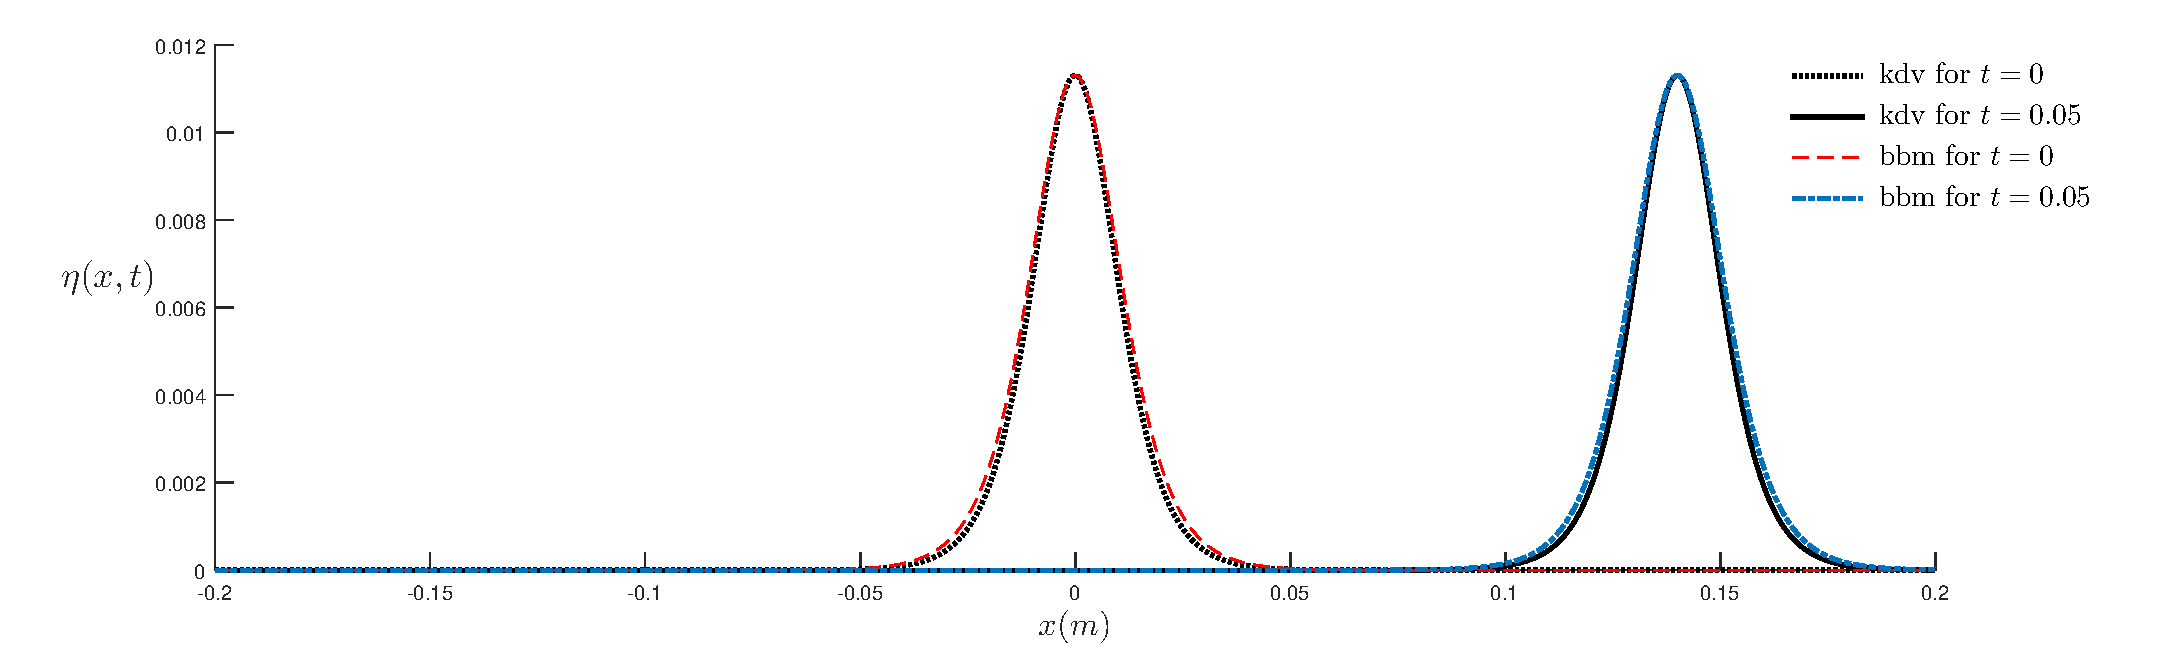
\includegraphics[width=\textwidth]{figs/KdVBBMSW.eps}
  \caption{\emph{Comparison of travelling-wave profiles generated by the KdV and BBM equations at several successive instants~$t$.}}
  \label{fig:2}
\end{figure}

The initial disturbance is a solitary wave of amplitude $A\,=\,0.0035$. The near-perfect overlap of the two families of curves at all reported times confirms that the BBM regularisation reproduces, to leading order, the dispersive and nonlinear balance captured by the KdV equation, thereby validating the asymptotic model for the haemodynamic parameters considered here. Figure~\ref{fig:2} juxtaposes the solitary-wave solutions obtained from the KdV and BBM models for a vessel of undisturbed radius $r_{\,0}=0.01\,\mathsf{m}$, wall thickness $h=3\times10^{-4}\,\mathsf{m}$, Young’s modulus $E=4.1\times10^{5}\,\mathsf{kg\,m^{-1}\,s^{-2}}$, wall density $\rho^{\;\omega}=10^{3}\,\mathsf{kg\,m^{-3}}$, and computational length $L=0.4\,\mathsf{m}$.

\subsubsection{Travelling-wave reduction of the cylindrical model}
\label{sec:cyl_travelling_wave}

In this Section, we derive exact solitary-wave solutions for the variable-coefficient cylindrical Boussinesq-type model \eqref{eq:bouss1}, \eqref{eq:bouss2}. The derivation follows the computer-algebra strategy of \cite{Dutykh2007}, implemented symbolically in \textsc{Maple}. We look for solutions that depend on a single travelling coordinate
\begin{equation*}
  \zeta \;\coloneqq\; x - c\,t,
\end{equation*}
so that
\begin{equation*}
  \bar{u}\,(x,t)\ =\ \bar{u}\,(\zeta), \qquad \eta\,(x,t)\ =\ \eta\,(\zeta), \qquad r^{\,w}\ =\ r_{\,0}+\eta, \qquad r_{\,0}=\text{const}.
\end{equation*}

\paragraph{Reduction of the governing equations.} Using the low-order approximation of the continuity \cref{eq:l6} together with the boundary condition \eqref{eq:kin}, one finds\footnote{Terms of order $\O\,(\delta^{\,4})$ and higher are consistently neglected throughout.}
\begin{equation*}
  \eta_{\,x t t}\ =\ -\,\Bigl(\,\frac{1}{2}\,r^{\,w}\,\bar{u}_{\,x}\ +\ r^{\,w}_{\,x}\,\bar{u}\,\Bigr)_{x t}\ +\ \O\,(\delta^{\,2}).
\end{equation*}
Substituting this expression into \cref{eq:5.2} yields the cylindrical Boussinesq system
\begin{align}
  \eta_{\,t}
  &\;+\; \frac{r_{\,0}}{2}\,\bar{u}_{\,x}
       \;+\;\frac{\eps}{2}\,\eta\,\bar{u}_{\,x}
       \;+\;\eps\,\eta_{\,x}\,\bar{u}
       \;-\;\frac{\delta^{\,2}}{48}\,r_{\,0}^{\,3}\,\bar{u}_{\,xxx}
       =\O\,\bigl(\delta^{\,4},\eps\,\delta^{\,2}\bigr), 
  \label{eq:bousnew1}\\
  \bar{u}_{\,t}
  &\;+\;\eps\,\bar{u}\,\bar{u}_{\,x}
       \;-\;\frac{\alpha\,r_{\,0}}{2}\,\delta^{\,2}\,\bar{u}_{\,xxt}
       \;+\;\beta\,\eta_{\,x}
       \;+\;\delta^{\,2}\,\beta\,\gamma\,\eta_{\,x t}
       \;-\;\frac{\delta^{\,2}}{6}\,r_{\,0}^{\,2}\,\bar{u}_{\,xxt}
       =\O\,\bigl(\delta^{\,4},\eps\,\delta^{\,2}\bigr).
  \label{eq:bousnew2}
\end{align}
Henceforth, we set $\gamma = 0$ (the purely elastic wall case). Introducing the convenience coefficients
\begin{equation*}
  a=\frac{r_{\,0}}{2}, \qquad  
  b=\frac{r_{\,0}^{\,3}}{48}, \qquad
  d=\frac{\alpha\,r_{\,0}}{2}, \qquad
  e=\beta, \qquad
  f=\frac{r_{\,0}^{\,2}}{6},
\end{equation*}
and rewriting \cref{eq:bousnew1,eq:bousnew2} in the travelling frame leads, after one integration with respect to~$\zeta$, to the coupled third-order ODE system
\begin{align}
  c\,\eta^{\,\prime}
  &\;+\;a\,\bar{u}^{\,\prime}
       \;+\;\frac{\eps}{2}\,\eta\,\bar{u}^{\,\prime}
       \;+\;\eps\,\eta^{\,\prime}\,\bar{u}
       \;-\;\delta^{\,2}\,b\,\bar{u}^{\,\prime\prime\prime}
       \;=\;0,
  \label{eq:5.9a} \\
  c\,\bar{u}^{\,\prime}
  &\;+\;\eps\,\bar{u}\,\bar{u}^{\,\prime}
       \;-\;\delta^{\,2}\,d\,c\,\bar{u}^{\,\prime\prime\prime}
       \;+\;e\,\eta^{\,\prime}
       \;-\;\delta^{\,2}\,f\,c\,\bar{u}^{\,\prime\prime\prime}
       \;=\;0,
  \label{eq:5.10a}
\end{align}
where primes denote differentiation with respect to~$\zeta$. Because solitary waves are spatially localised, all dependent variables and their derivatives vanish as $\zeta\ \to\ \pm\infty\,$.

\paragraph{Proportional flow ansatz.} Guided by extensive numerical experimentation, we set
\begin{equation}\label{eq:5.11a}
  \bar{u}\,(\zeta)\ =\ A\,\eta\,(\zeta)\,,
\end{equation}
where the proportionality constant $A$ will be determined self-consistently. Substituting \cref{eq:5.11a} into \cref{eq:5.9a,eq:5.10a}, integrating once under the zero-boundary conditions, and collecting like terms gives the pair
\begin{align}
  (c+aA)\,\eta \;-\;\delta^{\,2}\,b\,A\,\eta^{\,\prime\prime}\ &=\ -\frac{3}{4}\,\eps\,A\,\eta^{\,2}, \label{eq:5.13} \\
  (cA+e)\,\eta \;-\;\delta^{\,2}\,cA\,(d+f)\,\eta^{\,\prime\prime}\ &=\ -\frac{1}{2}\,\eps\,A^{\,2}\,\eta^{\,2}. \label{eq:5.14}
\end{align}
Demanding that the algebraic factors multiplying $\eta$ and $\eta^{\,\prime\prime}$ coincide in \cref{eq:5.13,eq:5.14} (otherwise only the trivial solution $\eta\equiv0$ would be admissible) yields the linear system
\begin{equation}\label{eq:compat}
  2Ac\ +\ 2aA^{\,2}\ =\ 3Ac\ +\ 3e\,, \qquad -Ac\ +\ 2aA^{\,2}\ =\ 3e\,,
\end{equation}
whose unique positive solution is\footnote{The positive root is selected to guarantee a right-propagating pulse ($c>0$).}
\begin{equation*}
  A^{\,2}\ =\ \frac{9\,e\,(d+f)}{6\,a\,(d+f)\ -\ 2\,b}, \qquad c\ =\ \frac{2\,b}{3\,(d+f)}\,A.
\end{equation*}
Restoring the original parameters,
\begin{equation*}
  A\ =\ 6\,\sqrt{\frac{\beta\,(3\alpha+1)}{r_{\,0}\,(36\alpha+11)}}, \qquad
  c\ =\ \frac{r_{\,0}}{6\alpha+2}\,\sqrt{\frac{\beta\,(3\alpha+1)}{r_{\,0}\,(36\alpha+11)}}\,.
\end{equation*}

\paragraph{Scalar solitary wave equation.} With the compatibility conditions \eqref{eq:compat} enforced, either of the relations \eqref{eq:5.13}, \eqref{eq:5.14} becomes
\begin{equation}
  A_{\,1}\,\eta^{\,\prime}
  \;-\;
  B_{\,1}\,\eta^{\,\prime\prime\prime}
  \;=\;
  \eta\,\eta^{\,\prime},
  \qquad
  A_{\,1}:=\frac{4be+6ae(d+f)}{9e(d+f)\,\eps},
  \quad
  B_{\,1}:=\frac{2b\,\delta^{\,2}}{3\,\eps},
  \label{eq:lem}
\end{equation}
which is a well-known integrable third-order ODE of the KdV type \cite{Newell1977}.  Provided $A_{\,1}B_{\,1}>0$, equation \eqref{eq:lem} admits the classical $\sech^{2}$ solitary-wave solution:
\begin{equation*}
  \eta(\zeta)\ =\ 3\,A_{\,1}\,
  \sech^{2}\,\Bigl[
    \frac12\,\sqrt{A_{\,1}/B_{\,1}}\;(\zeta-\zeta_{\,0})
  \Bigr], \qquad \zeta_{\,0}\ \in\ \R.
\end{equation*}
Re-expressed through the physical parameters,
\begin{equation}
  \eta(\zeta)\ =\ -\,\frac{3\,r_{\,0}\,(7+18\alpha)}{54\alpha+18}\,
  \sech^{2}\,\Bigl[\frac{\zeta}{2\delta}\,\sqrt{\frac{28+72\alpha}{r_{\,0}^{\,2}(3\alpha+1)}}\Bigr], \label{eq:solitarybouss1}
\end{equation}
and, by virtue of \eqref{eq:5.11},
\begin{equation}
  \bar{u}(\zeta)\ =\ \frac{r_{\,0}\,(7+18\alpha)}{3\alpha+1}\,
  \sqrt{\frac{\beta\,(3\alpha+1)}{r_{\,0}\,(36\alpha+11)}}\,
  \sech^{2}\,\Bigl[\frac{\zeta}{2\delta}\,\sqrt{\frac{28+72\alpha}{r_{\,0}^{\,2}(3\alpha+1)}}\Bigr]. \label{eq:solitarybouss2}
\end{equation}
The entire derivation has been cross-checked symbolically in \textsc{Maple}; the annotated worksheet is provided in the accompanying codes repository.

\section{Dispersion relations}
\label{sec:disp}

We first examine the linear dispersion characteristics of the full three-dimensional model and compare them with those obtained from the linearised Euler equations by following \cite{Mitsotakis2018}:
\begin{equation}\label{eq:lin_u}
  u_{\,t}\;+\;\frac{1}{\rho}\,p_{\,x}\;=\;0,
\end{equation}
\begin{equation}\label{eq:lin_v}
  v_{\,t}\;+\;\frac{1}{\rho}\,p_{\,r}\;=\;0,
\end{equation}
\begin{equation}\label{eq:lin_cont}
  u_{\,x}\;+\;v_{\,r}\;+\;\frac{1}{r}\,v\;=\;0,
\end{equation}
subject to the boundary conditions
\begin{equation}\label{eq:lin_bc_kin}
  v\,\left(x,r^{\,w},t\right)\;=\;\eta_{\,t}\,\left(x,t\right), 
\end{equation}
\begin{equation}\label{eq:lin_bc_dyn}
  p^{\,w}\,\left(x,t\right)\; = \;\rho^{\,w}h\,\eta_{\,tt}\,\left(x,t\right)\; + \;\frac{E\,h}{\rho_{\,0}^{\,2}}\,
  \eta\,\left(x,t\right),
\end{equation}
\begin{equation}\label{eq:lin_bc_axis}
  v\,\left(x,0,t\right)\; = \;0.
\end{equation}

\paragraph{Normal-mode ansatz.} We consider normal modes of the form
\begin{equation*}
  u\,\left(x,r,t\right)=u_{\,0}\left(r\right)\exp\,\bigl(\ui\left(kx-\omega t\right)\bigr),\qquad
  v\,\left(x,r,t\right)=v_{\,0}\left(r\right)\exp\,\bigl(\ui\left(kx-\omega t\right)\bigr),
\end{equation*}
\begin{equation*}
  \eta\,\left(x,t\right)=\eta_{\,0}\exp\,\bigl(\ui\left(kx-\omega t\right)\bigr),\qquad
  p\,\left(x,r,t\right)=p_{\,0}\left(r\right)\exp\,\bigl(\ui\left(kx-\omega t\right)\bigr),
\end{equation*}
and substitute these expressions into the linearised Euler system. The axial velocity amplitude $u_{\,0}\left(r\right)$ then satisfies the modified Bessel equation
\begin{equation}\label{eq:lin_bessel}
  r\,u_{\,0}^{\,\prime\prime}\left(r\right)\;+\;u_{\,0}^{\,\prime}\left(r\right)\;-\;r\,k^{\,2}\,
  u_{\,0}\left(r\right)\;=\;0,
\end{equation}
together with the regularity condition
\begin{equation}\label{eq:lin_bc_centre}
  u_{\,0}^{\,\prime}\left(0\right)\;=\;0
\end{equation}
and the wall conditions
\begin{align}
  u_{\,0}^{\,\prime}\left(r_{\,0}\right) & \;=\;\omega k\,\eta_{\,0}, \label{eq:lin_bc_wall_kin}\\
  \rho^{\,w}h\,\omega^{\,2}\,\eta_{\,0} & \;+\;\frac{\rho\omega}{k}\,u_{\,0}\left(r_{\,0}\right)
  \;-\;\frac{E\,h}{r_{\,0}^{\,2}}\,\eta_{\,0}\;=\;0.
  \label{eq:lin_bc_wall_dyn}
\end{align}
The Bessel problem \eqref{eq:lin_bessel}--\eqref{eq:lin_bc_wall_kin} admits the solution
\[
  u_{\,0}\left(r\right)\;=\;\eta_{\,0}\,\omega\,
  \frac{I_{\,0}\left(kr\right)}{I_{\,1}\left(kr_{\,0}\right)},
\]
where $I_{\,0}$ and $I_{\,1}$ are the modified Bessel functions of the first kind.  Inserting this expression into \eqref{eq:lin_bc_wall_dyn} yields the \emph{exact} linear dispersion relation
\begin{equation}\label{eq:disp_euler}
  \omega_{\,\eps}^{\,2}\left(k\right)\;=\;
  \frac{E\,h}{\rho\,r_{\,0}^{\,3}}\,
  \frac{r_{\,0}k\,I_{\,1}\left(kr_{\,0}\right)}
       {\displaystyle\frac{\rho^{\,w}h}{\rho r_{\,0}}\,
       r_{\,0}k\,I_{\,1}\left(kr_{\,0}\right)\;+\;I_{\,0}\left(kr_{\,0}\right)}.
\end{equation}

\paragraph{Reduced Boussinesq system.} We next linearise the depth-averaged system \eqref{eq:5.1}--\eqref{eq:5.2} and again insert the normal-mode ansatz.  This procedure leads to
\begin{align}
  \frac{r_{\,0}}{2}\,\ui k\,\bar{u}_{\,0}\;-\;\ui\omega\,\eta_{\,0}
  &\;-\;\frac{\delta^{\,2}}{48}\,r_{\,0}^{\,3}\,(\ui k)^{3}\bar{u}_{\,0}
  \;=\;0, \label{eq:lin_red1}\\
  -\ui\omega\,\bar{u}_{\,0}
  &\;-\;\alpha\delta^{\,2}\,k\omega^{\,2}\eta_{\,0}
  \;+\;\ui k\,\beta\,\eta_{\,0}
  \;+\;\delta^{\,2}\,\beta\gamma\,(\ui k)\omega\,\eta_{\,0}
  \;+\;\frac{\delta^{\,2}}{6}\,r_{\,0}^{\,2}\,k^{\,2}\omega\,\bar{u}_{\,0}
  \;=\;0. \label{eq:lin_red2}
\end{align}
Elimination of $\bar{u}_{\,0}$ gives the quadratic dispersion relation
\begin{equation}\label{eq:disp_bous}
  \Bigl(24\,r_{\,0}k\;+\;r_{\,0}^{\,3}k^{\,3}\Bigr)\Bigl(\alpha k\;+\;
  \frac{48\;+\;8\,\delta^{\,2}r_{\,0}^{\,2}k^{\,2}}{24\,r_{\,0}k\;+\;r_{\,0}^{\,3}k^{\,3}}\Bigr)\omega^{\,2}
  \;+\;\ui\,\delta^{\,2}\,\beta\gamma\,k\,\omega\;-\;\beta\,k\;=\;0.
\end{equation}

\paragraph{Modified Boussinesq system.} For the refined system \eqref{eq:bousnew1}--\eqref{eq:bousnew2} we proceed analogously and obtain the alternate quadratic
\begin{equation}\label{eq:disp_mod_bous}
  \Bigl(24\,r_{\,0}k\;+\;\delta^{\,2}r_{\,0}^{\,3}k^{\,3}\Bigr)
  \bigl(-48\;-\;24\,\alpha\delta^{\,2}r_{\,0}^{\,2}k^{\,2}\;
  -\;8\,\delta^{\,2}r_{\,0}^{\,2}k^{\,2}\bigr)\omega^{\,2}
  \;-\;\ui\,\delta^{\,2}\,\beta\gamma\,k\,\omega
  \;+\;\beta\,k\;=\;0.
\end{equation}

\paragraph{Comparison of phase speeds.} The phase speeds furnished by \eqref{eq:disp_euler}, \eqref{eq:disp_bous} and \eqref{eq:disp_mod_bous}, together with those of the classical KdV and BBM reductions, are depicted in \cref{fig:disp} for
\[
  r_{\,0}=0.01\,\mathsf{m}, \qquad
  h=3\times10^{-4}\,\mathsf{m}, \qquad
  E=4.1\times10^{\,5}\,\mathsf{kg}\,\mathsf{m}^{-1}\,\mathsf{s}^{-2}, \qquad
  \rho^{\,\omega}=10^{3}\,\mathsf{kg}\,\mathsf{m}^{-3}, \qquad
  \rho=1060\,\mathsf{kg}\,\mathsf{m}^{-3}.
\]

\begin{figure}[t]
  \centering
  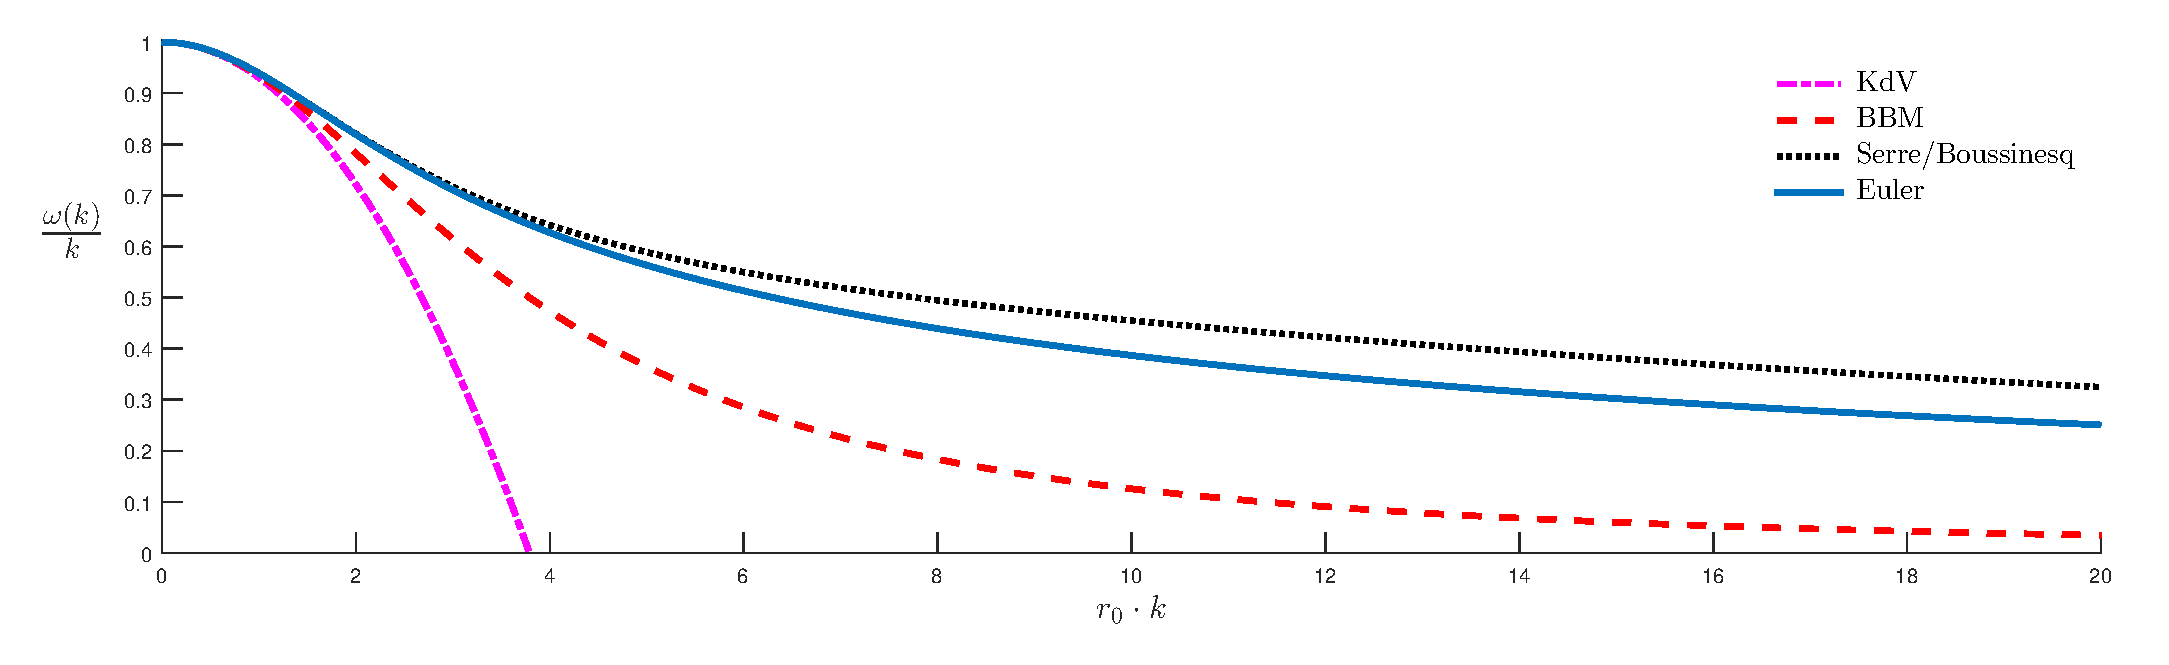
\includegraphics[width=\textwidth]{figs/disp1.eps}
  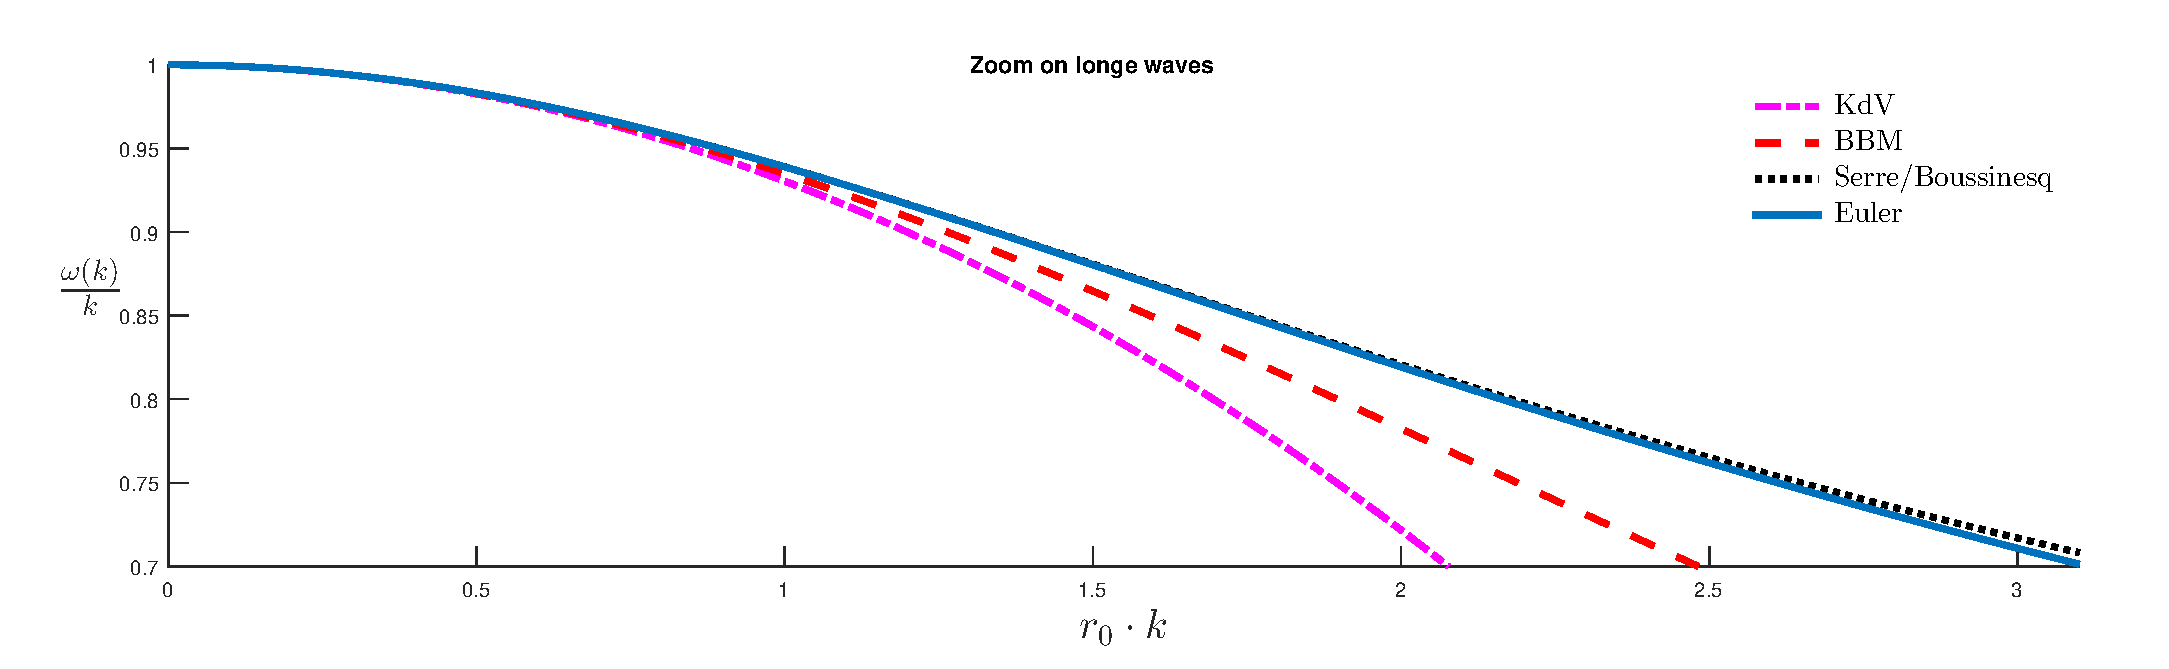
\includegraphics[width=\textwidth]{figs/disp4.eps}
  \caption{\em Comparison of linear phase speeds predicted by various Boussinesq-type approximations with the reference Euler result.}
  \label{fig:disp}
\end{figure}

\paragraph{Remarks.} The algebraic relations \eqref{eq:disp_bous} and \eqref{eq:disp_mod_bous} demonstrate that both the classical and the modified depth-averaged models reproduce the low-frequency branch of the exact dispersion curve with the correct slope.  The modified formulation retains this agreement while reducing the high-frequency error introduced by the classical Boussinesq truncation, thereby reinforcing its suitability for simulating arterial pulse waves over physiologically relevant wavelengths.

\section{Stokes expansions}

In this section, we employ Stokes expansion techniques to analyze the nonlinear wave solutions of our derived models. Stokes expansions provide a systematic approach to construct periodic wave solutions in weakly nonlinear regimes, revealing how nonlinearity affects the dispersion relation and wave profiles. We will focus particularly on applying this methodology to the KdV and BBM reductions of our cylindrical Boussinesq system, demonstrating how the interplay between nonlinearity and dispersion shapes the propagation characteristics of arterial pulse waves. This analysis will further elucidate the amplitude-dependent modifications to wave speed and structure that are essential for accurately modeling blood flow dynamics in elastic vessels.

\subsection{Weakly nonlinear Stokes expansion for the KdV reduction}

Stokes' pioneering investigations of periodic gravity waves, first published in 1847, revealed two fundamental facts that remain central to non-linear dispersive‐wave theory: \textit{(i)} coherent periodic wave-trains are admissible even when the governing equations are non-linear, and \textit{(ii)} the dispersion relation acquires an explicit dependence on the wave amplitude. The latter feature gives rise to qualitatively new phenomena rather than mere numerical corrections.

We apply Stokes' method to the KdV reduction
\begin{equation}\label{eq:kdv_red}
  \eta_{t}
  +\tilde{c}\,\eta_{x}
  +\frac{5}{2}\frac{\tilde{c}}{r_{0}}\,
   \eta\,\eta_{x}
  +\frac{\tilde{c}\,(12\tilde{\alpha}+3r_{0})\,r_{0}}{48}\,
   \eta_{xxx}
  =0,
\end{equation}
obtained by setting $\gamma=0$ in \eqref{eq:KdVdim}. Introducing the small parameter $\varepsilon$ and the travelling phase
\(
  \theta=kx-\omega t,
\)
we seek an expansion
\begin{equation}\label{eq:stokes_ansatz}
  \frac{\eta}{r_{0}}
  =\varepsilon\,\xi_{1}(\theta)
   +\varepsilon^{2}\,\xi_{2}(\theta)
   +\varepsilon^{3}\,\xi_{3}(\theta)
   +\dots.
\end{equation}
With the abbreviations
\[
  a=\tilde{c},\qquad
  b=\frac{5\tilde{c}}{2r_{0}},\qquad
  c=\frac{\tilde{c}\,(12\tilde{\alpha}+3r_{0})\,r_{0}}{48},
\]
equation \eqref{eq:kdv_red} yields the hierarchy
\begin{align}
  (\omega-ak)\,\xi_{1}'-c\,k^{3}\,\xi_{1}''' &=0, \label{eq:h1}\\
  (\omega-ak)\,\xi_{2}'-c\,k^{3}\,\xi_{2}''' &=-b\,k\,\xi_{1}\,\xi_{1}',
             \label{eq:h2}\\
  (\omega-ak)\,\xi_{3}'-c\,k^{3}\,\xi_{3}'''
     &=-b\,k\bigl(\xi_{1}^{2}\bigr)'
       -\omega_{2}\,\xi_{1}', \label{eq:h3}
\end{align}
where
\(
  \omega=\omega_{0}(k)+\varepsilon^{2}\omega_{2}(k)+\dots
\)
and
\(
  \omega_{0}(k)=ak-ck^{3}.
\)
Equation \eqref{eq:h1} admits the normalised solution
\(
  \xi_{1}(\theta)=\cos\theta.
\)
Solving \eqref{eq:h2} with this choice gives
\[
  \xi_{2}(\theta)=\frac{b}{12\,c\,k^{2}}\cos(2\theta).
\]
The right-hand side of \eqref{eq:h3} contains a resonant term
proportional to $\sin\theta$; eliminating it fixes
\(
  \displaystyle
  \omega_{2}(k)=\frac{b^{2}}{24\,c\,k}.
\)
A particular solution of \eqref{eq:h3} is then
\(
  \displaystyle
  \xi_{3}(\theta)=\frac{b^{2}}{192\,c^{2}\,k^{4}}\cos(3\theta).
\)
The above sequence of calculations can be summarized in the form of the following theorem, which provides a closed-form expression for the periodic wave solution and the corresponding nonlinear dispersion relation up to third order in the perturbation parameter.

\begin{theorem}\label{thm:stokes_periodic}
Let $\varepsilon\ll1$ and let $k>0$ be fixed.  To third order in $\varepsilon$ the KdV equation \eqref{eq:kdv_red} possesses a $2\pi/k$-periodic Stokes wave of the form
\begin{equation}\label{eq:eta_series}
  \frac{\eta}{r_{0}}
  =\varepsilon\cos\theta
  +\varepsilon^{2}\frac{b}{12\,c\,k}\cos(2\theta)
  +\varepsilon^{3}\frac{b^{2}}{192\,c^{2}\,k^{4}}\cos(3\theta)
  +\O(\varepsilon^{4}),
  \qquad
  \theta=kx-\omega t,
\end{equation}
where the non-linear dispersion relation is
\begin{equation}\label{eq:disp_relation}
  \omega(k,\varepsilon)
  =ak-ck^{3}
  +\varepsilon^{2}\frac{b^{2}}{24\,c\,k}
  +\O(\varepsilon^{4}).
\end{equation}
The phase speed thus increases quadratically with amplitude, demonstrating the amplitude-dependent dispersion characteristic of Stokes waves.
\end{theorem}

Theorem~\ref{thm:stokes_periodic} recovers the classical Stokes expansion for the KdV equation, with coefficients determined by the underlying physical parameters $\tilde{c}$, $\tilde{\alpha}$, and $r_{0}$. The result confirms that even weak non-linearity modifies the linear dispersion relation by an $\O(\varepsilon^{2})$ term proportional to the square of the wave amplitude.

\subsection{Weakly nonlinear Stokes expansion for the BBM reduction}

Consider the Benjamin-Bona-Mahony (BBM) reduction obtained from the long-wave model,
\begin{equation}\label{eq:BBM}
  \eta_{t}
  +\tilde{c}\,\eta_{x}
  +\frac{5\tilde{c}}{2r_{0}}\,\eta\,\eta_{x}
  -\frac{(12\tilde{\alpha}+3r_{0})\,r_{0}}{48}\,\eta_{xxt}
  =0,
\end{equation}
where, for simplicity, $\gamma=0$ has been set.  Denoting
\[
  a^{\ast}=\tilde{c},\qquad
  b^{\ast}=\frac{5\tilde{c}}{2r_{0}},\qquad
  c^{\ast}=\frac{\tilde{c}(12\tilde{\alpha}+3r_{0})\,r_{0}}{48},
\]
we expand the solution in a Stokes series,
\begin{equation}\label{eq:bbm_ansatz}
  \frac{\eta}{r_{0}}
  =\varepsilon\,\xi_{1}(\theta)
   +\varepsilon^{2}\,\xi_{2}(\theta)
   +\varepsilon^{3}\,\xi_{3}(\theta)
   +\dots,
  \qquad
  \theta=kx-\omega t,
\end{equation}
with $\varepsilon \ll 1$.

\paragraph{Hierarchy of amplitude equations.} Insertion of \eqref{eq:bbm_ansatz} into \eqref{eq:BBM} gives, at successive orders in $\varepsilon$,
\begin{align}
  (\omega-a^{\ast}k)\,\xi_{1}'-c^{\ast}\,\omega\,k^{2}\,\xi_{1}''' &=0,\label{eq:bbm_h1}\\
  (\omega-a^{\ast}k)\,\xi_{2}'-c^{\ast}\,\omega\,k^{2}\,\xi_{2}''' &=b^{\ast}k\,\xi_{1}\xi_{1}',\label{eq:bbm_h2}\\
  (\omega-a^{\ast}k)\,\xi_{3}'-c^{\ast}\,\omega\,k^{2}\,\xi_{3}''' &=b^{\ast}k\,(\xi_{1}^{2})'
          -\omega_{2}\,\xi_{1}'
          +c^{\ast}\omega_{2}k^{2}\,\xi_{1}'''.  \label{eq:bbm_h3}
\end{align}
The dispersion relation is again expanded as
\[
  \omega(k,\varepsilon)
  =\omega_{0}(k)+\varepsilon^{2}\,\omega_{2}(k)+\dots,
  \qquad
  \omega_{0}(k)=\frac{a^{\ast}k}{1+c^{\ast}k^{2}}.
\]
Taking $\omega_{1}=0$ eliminates secular terms at $\O(\varepsilon)$.

\paragraph{First‐ and second‐order solutions.} Equation \eqref{eq:bbm_h1} admits the normalised solution
\[
  \xi_{1}(\theta)=\cos\theta.
\]
Solving \eqref{eq:bbm_h2} for $\xi_{2}$ gives
\begin{equation}\label{eq:bbm_xi2}
  \xi_{2}(\theta)
  =\frac{b^{\ast}(1+c^{\ast}k^{2})}{12\,a^{\ast}c^{\ast}k^{2}}
   \cos(2\theta).
\end{equation}

\paragraph{Elimination of resonances at third order.} The right-hand side of \eqref{eq:bbm_h3} contains the resonant term
\(
  \propto\sin\theta.
\)
Choosing
\begin{equation}\label{eq:bbm_omega2}
  \omega_{2}(k)=\frac{b^{\ast\,2}}{24\,c^{\ast}k},
\end{equation}
cancels this term. Integrating once then yields
\begin{equation}\label{eq:bbm_xi3}
  \xi_{3}(\theta)
  =\frac{b^{\ast\,2}(1+c^{\ast}k^{2})}{192\,c^{\ast\,2}k^{4}}
   \cos(3\theta).
\end{equation}

The above sequence of calculations can be summarized in the form of the following theorem, which provides a closed-form expression for the periodic wave solution and the corresponding nonlinear dispersion relation up to third order in the perturbation parameter.
\begin{theorem}\label{thm:bbm_stokes}
Let $\varepsilon\ll1$ and $k>0$. The BBM equation \eqref{eq:BBM} possesses a $2\pi/k$-periodic Stokes wave of the form
\begin{equation}\label{eq:bbm_eta_series}
  \frac{\eta}{r_{0}}
  =\varepsilon\cos\theta
   +\varepsilon^{2}
      \frac{b^{\ast}(1+c^{\ast}k^{2})}{12\,a^{\ast}c^{\ast}k^{2}}
      \cos(2\theta)
   +\varepsilon^{3}
      \frac{b^{\ast\,2}(1+c^{\ast}k^{2})}{192\,c^{\ast\,2}k^{4}}
      \cos(3\theta)
   +\O(\varepsilon^{4}), \qquad \theta=kx-\omega t,
  \end{equation}
where the non‐linear dispersion relation is
\begin{equation}\label{eq:bbm_dispersion}
  \omega(k,\varepsilon)
  =\frac{a^{\ast}k}{1+c^{\ast}k^{2}}
   +\varepsilon^{2}\frac{b^{\ast\,2}}{24\,c^{\ast}k}
   +\O(\varepsilon^{4}).
\end{equation}
Consequently, the phase speed obeys
\(
  c_{\mathrm{ph}}=\omega/k
\)
and increases quadratically with the wave amplitude, reflecting the weakly non-linear character of the BBM model.
\end{theorem}

Theorem~\ref{thm:bbm_stokes} mirrors the result obtained earlier for the KdV equation, but with the BBM-specific linear dispersion
\(
  \omega_{0}(k)=a^{\ast}k/(1+c^{\ast}k^{2})
\)
and modified amplitude coefficients. Together with Theorem~\ref{thm:stokes_periodic}, it emphasises that both the KdV and BBM reductions support periodic Stokes waves whose speeds are augmented by non-linearity, thereby enriching the spectrum of observable dynamics in pulsatile blood-flow models.

\section{Conservation laws and symmetries}
\label{sec:cons_sym}

Every transformation that maps the solution manifold of a system of differential equations (DEs) into itself is termed a \emph{symmetry}. The classical Lie method furnishes a systematic procedure for constructing single- and multi-parameter Lie groups of point symmetries and has been successfully employed for algebraic, ordinary, and partial differential equations \cite{Cheviakov2007}. Analogous computational frameworks exist for the determination of contact and higher-order symmetries, as well as for non-local symmetries. Closely related methodologies have been developed for approximate symmetries, symmetries of difference schemes, and those of integro-differential equations; see, for instance, the extensive compendium in \cite{Ibragimov1995}.

Information about a PDE system's conservation laws is indispensable for a profound understanding of its symmetry structure. Conservation laws encode the fundamental physical invariants of the underlying process and underpin analytical results on existence, uniqueness, and stability \cite{Olver1993, Evans2010}. They likewise play a pivotal rôle in geometric analyses of solution manifolds \cite{Bluman1987} and in the design of robust numerical schemes that preserve key physical quantities \cite{LeVeque2002}.

In this section we introduce the recently developed \textsc{Maple} package \texttt{GeM} \cite{Cheviakov2007}. The package provides fully automated routines for the local symmetry analysis of ODEs and PDEs and for the systematic search of conservation laws.  All determining equations are generated symbolically in a form amenable to efficient automatic reduction and solution.

\subsection{Conservation laws}\label{ssec:CL}

Divergence expressions that vanish on the solution set of a PDE system represent its \emph{local conservation laws}.  
Such laws arise ubiquitously: classical examples include the conservation of mass, momentum, charge, and energy. For time-dependent systems on bounded domains they yield first integrals, while for ODEs they provide conserved quantities \cite{Cheviakov2010}. Conservation laws play a decisive rôle in the analytical theory of nonlinear PDEs, notably in the study of stability and in the construction of numerical schemes \cite{Lax1968, Knops1984}. Moreover, a local conservation law often serves to introduce non-local (potential) variables, thereby generating auxiliary PDE systems with identical solution sets \cite{Bluman1987, Sjoberg2004}.

The four standard flux-construction techniques, together with the direct method for conservation-law derivation, have all been implemented symbolically in \texttt{GeM} \cite{Cheviakov2007}.  Package routines return the determining equations in a form suitable for automatic reduction and solution. They are capable of treating high-order systems with numerous dependent and independent variables and can typically be executed on a standard desktop computer.

Consider an $N$-equation PDE system of order $K$ for
\[
  x=(x^{1},\dots,x^{n}),\qquad
  u(x)=(u^{1}(x),\dots,u^{m}(x)),
\]
written compactly as
\begin{equation}\label{eq:chap4.1}
  L^{\sigma}[u]\;=\;L^{\sigma}\bigl(x,u,\partial u,\dots,\partial^{K}u\bigr)\;=\;0,
  \qquad \sigma \in \{1,\dots,N\}.
\end{equation}
We denote first-order derivatives by
\[
  u^{\nu}_{\,i}\;=\;\pd{u^{\nu}}{x^{i}}, 
\]
and collect all derivatives of order~$p$ in
\begin{equation}\label{eq:chap4.7}
  \partial^{p}u\;=\;
  \Bigl\{\,
      \partial_{x^{i_{1}}\dots x^{i_{p}}} u^{\nu} \,\bigm|\,
      \nu \in \{1,\dots,m\},\;
      i_{1},\dots,i_{p} \in \{1,\dots,n\}
  \Bigr\}.
\end{equation}
A \emph{solved form} of \eqref{eq:chap4.1} is obtained when
\begin{equation}\label{eq:chap4.5}
  L^{\sigma}[u]\;=\;
  u^{\,j_{\sigma}}_{\,i_{\sigma,1}\dots i_{\sigma,s}}
  \;-\;
  M^{\sigma}\bigl(x,u,\partial u,\dots,\partial^{K}u\bigr)
  \;=\;0,
  \qquad
  \sigma=1,\dots,N,
\end{equation}
where $1\leq j_{\sigma}\leq m$, $s\leq K$, and $1\leq i_{\sigma,k}\leq n$. The set $\{u^{\,j_{\sigma}}_{\,i_{\sigma,1}\dots i_{\sigma,s}}\}_{\sigma=1}^{N}$ contains $N$ linearly independent leading derivatives that do not appear in the right-hand sides $M^{\sigma}$.

\paragraph{Total and Euler operators.} The total derivative with respect to $x^{i}$ is
\[
  D_{i}\;=\;
  \pd{}{x^{i}}
  \;+\;
  u^{\nu}_{\,i}\pd{}{u^{\nu}}
  \;+\;
  u^{\nu}_{\,ii_{1}}\pd{}{u^{\nu}_{\,i_{1}}}
  \;+\;
  u^{\nu}_{\,ii_{1}i_{2}}\pd{}{u^{\nu}_{\,i_{1}i_{2}}}
  \;+\;\dots,
  \qquad i \in \{1,\dots,n\}.
\]
The Euler operator acting on a differential function $U(x)$ is
\begin{equation}\label{eq:chap4.4}
  E_{U}\;=\;
  \pd{}{U}
  \;-\;
  D_{i}\pd{}{U_{\,i}}
  \;+\;
  \dots
  \;+\;
  (-1)^{s}\,D_{i_{1}}\dots D_{i_{s}}
  \pd{}{U_{\,i_{1}\dots i_{s}}}
  \;+\;\dots
\end{equation}

\paragraph{Local conservation laws.} A divergence expression
\begin{equation}\label{eq:chap4.2}
  \operatorname{div}\Phi
  \;\equiv\;
  D_{i}\,\phi^{i}[u]
  \;=\;
  D_{1}\phi^{1}
  \;+\;\dots\;+\;
  D_{n}\phi^{n}
  \;=\;0
\end{equation}
valid on the solution set of~\eqref{eq:chap4.1} is called a local conservation law. The fluxes $\phi^{i}$ may depend on $x$, $u$, and finitely many derivatives of~$u$.

A conservation law \eqref{eq:chap4.2} is \emph{trivial} if
\[
  \phi^{i}\;=\;A^{i}[u]\;+\;D_{j}H^{ij}[u],
\]
where $A^{i}$ vanishes on solutions of~\eqref{eq:chap4.1} and $\operatorname{div}H \equiv 0$ identically.

\paragraph{Direct construction by multipliers.} Non-trivial conservation laws arise from multipliers
$\{\Lambda_{\sigma}(x,U,\partial U,\dots,\partial^{\ell}U)\}_{\sigma=1}^{N}$ that satisfy
\begin{equation}\label{eq:chap4.3}
  \Lambda_{\sigma}[U]\,L^{\sigma}[U]
  \;\equiv\;
  D_{i}\,\phi^{i}[U],
\end{equation}
identically in the jet space. On any solution $U=u$ of~\eqref{eq:chap4.1} the right-hand side of \eqref{eq:chap4.3} vanishes, yielding a local conservation law. Completeness of the direct method has been established for broad classes of systems, including those in (generalised) Kovalevskaya form \cite{Olver1993}:
\begin{theorem}\label{thm:char_form}
  For every local conservation law $D_{i}\phi^{i}[u]=0$ of a system in solved form~\eqref{eq:chap4.5} there exists an equivalent conservation law whose fluxes contain no leading derivatives, viz.
  \[
      D_{i}\,\tilde{\phi}^{i}[U]
      \;=\;
      \widetilde{\Lambda}_{\sigma}[U]\,
      \bigl(
          U^{\,j_{\sigma}}_{\,i_{\sigma,1}\dots i_{\sigma,s}}
          -M^{\sigma}[U]
      \bigr),
  \]
  for some non-singular multipliers $\{\widetilde{\Lambda}_{\sigma}\}_{\sigma=1}^{N}$. The correspondence between conservation laws and multiplier sets is, however, not always one-to-one.
\end{theorem}

\paragraph{The \texttt{GeM} workflow.}
A typical sequence for conservation-law computation in \texttt{GeM} proceeds as follows:
\begin{enumerate}[label=(\roman*)]
  \item \textbf{Initialisation:}
        \verb|restart;|\\
        \verb|read("d:/gem32_12.mpl"):|\\
        \verb|with(GeM): with(linalg): with(DEtools): with(PDEtools):|
  \item \textbf{Declaration of variables:}\\
        \verb|gem_decl_vars(indeps=[...], deps=[...], freefunc=[...], freeconst=[...]);|
  \item \textbf{Input of the PDE system:}\\
        \verb|gem_decl_eqs([...], solve_for=[...]);|
  \item \textbf{Generation of determining equations:}\\
        \verb|det_eqs := gem_conslaw_det_eqs([...]);|
  \item \textbf{Selection of unknown multipliers:}\\
        \verb|CL_multipliers := gem_conslaw_multipliers();|
  \item \textbf{Reduction of the over-determined system:}\\
        \verb|simplified_eqs := DEtools[rifsimp](det_eqs, CL_multipliers, mindim=1);|
  \item \textbf{Solution of determining equations:}\\
        \verb|multipliers_sol := pdsolve(simplified_eqs[Solved]);|
  \item \textbf{Computation of fluxes:}\\
        \verb|gem_get_CL_fluxes(multipliers_sol);|
\end{enumerate}

\subsection{Symmetries}\label{ssec:symm}

A \emph{symmetry group} of a differential equation maps each solution to another solution. Continuous (Lie) symmetries are therefore inherent to every non-trivial system. The foundational concepts were introduced by \textsc{Sophus Lie} in the late nineteenth century and have since evolved into a versatile tool for analysing ODEs and PDEs.

For an $n$-dimensional independent variable $x$ and $m$-component dependent variable $u$, a one-parameter group of point transformations reads
\[
  (x')^{i}=f^{i}(x,u;\varepsilon), \qquad
  (u')^{\nu}=g^{\nu}(x,u;\varepsilon),
  \qquad
  i \in \{1,\dots,n\},\;
  \nu \in \{1,\dots,m\},
\]
or, in infinitesimal form,
\[
  (x')^{i}=x^{i}+\varepsilon\,\xi^{i}(x,u)+\mathcal{O}(\varepsilon^{2}),\qquad
  (u')^{\nu}=u^{\nu}+\varepsilon\,\eta^{\nu}(x,u)+\mathcal{O}(\varepsilon^{2}).
\]
The associated generator is
\[
  X=\xi^{i}(x,u)\,\pd{}{x^{i}}+\eta^{\nu}(x,u)\,\pd{}{u^{\nu}}.
\]
Its $K$-th prolongation is obtained via the standard formulae involving total derivatives $D_{i}$; cf. \eqref{eq:chap4.4}. The group is a symmetry of~\eqref{eq:chap4.1} iff
\[
  X^{(K)}\,L^{\sigma}=0
  \quad\text{whenever}\quad
  L^{\sigma}=0,
  \qquad \sigma \in \{1,\dots,N\}.
\]

\paragraph{The \texttt{GeM} workflow for symmetries.}
\begin{enumerate}[label=(\roman*)]
  \item \textbf{Initialisation.}
  \item \textbf{Declaration of variables and parameters.}
  \item \textbf{Input of the PDE system.}
  \item \textbf{Generation of determining equations:}\\
        \verb|det_eqs := gem_symm_det_eqs([...]);|
  \item \textbf{Selection of symmetry components:}\\
        \verb|sym_components := gem_symm_components();|
  \item \textbf{Reduction of the system:}\\
        \verb|simplified_eqs := DEtools[rifsimp](det_eqs, sym_components, mindim=1);|
  \item \textbf{Solution of determining equations:}\\
        \verb|symm_sol := pdsolve(simplified_eqs[Solved]);|
  \item \textbf{Output of symmetries:}\\
        \verb|gem_output_symm(symm_sol);|
\end{enumerate}

Detailed examples for both the Boussinesq and the full cylindrical blood-flow models are provided below, together with the resulting conservation laws, symmetry generators, and the corresponding one-parameter transformation groups.

\paragraph{Conservation laws and symmetries for the Boussinesq system.}

For the cylindrical Boussinesq system \eqref{eq:bouss1}, \eqref{eq:bouss2} with constant radius $r_{0}$, a direct multiplier search yields the local conservation law
\begin{multline}
  \Bigl[\,\bar{u}
         +\frac{1}{2}\,\tilde{\beta}\,\gamma\,\eta_{x}
         +\frac{2}{3}\,\tilde{\alpha}\,\eta_{xt}
         -\frac{1}{18}\,r_{0}^{2}\,\bar{u}_{xx}\Bigr]_{t}
  +\Bigl[\,\frac{1}{2}\,\bar{u}^{2}
        +\tilde{\beta}\,\eta
        +\frac{1}{2}\,\tilde{\beta}\,\gamma\,\eta_{t}
        -\frac{1}{9}\,r_{0}^{2}\,\bar{u}_{tx}
        +\frac{1}{3}\,\tilde{\alpha}\,\eta_{tt}\Bigr]_{x}=0 .
\end{multline}
Here $\tilde{\alpha}= \mathsf{\rho^{w}\,h/\rho}$ and
$\tilde{\beta}(x)=\mathsf{E\,h/(\rho\,r_{0}^{2})}$.  
The corresponding multipliers are
\begin{itemize}
  \item $\lambda_{1}(t,x,\eta,\bar{u},\dots)=0$,
  \item $\lambda_{2}(t,x,\eta,\bar{u},\dots)=1$.
\end{itemize}

The infinitesimal symmetry generators are
\[
  X_{1}=\partial_{x},
  \qquad
  X_{2}=\partial_{t},
\]
with associated point transformations
\[
  x' = x+\varepsilon_{1},
  \quad
  t' = t,
  \quad
  \eta'=\eta,
  \quad
  \bar{u}'=\bar{u};
  \qquad
  x' = x,
  \quad
  t' = t+\varepsilon_{2},
  \quad
  \eta'=\eta,
  \quad
  \bar{u}'=\bar{u}.
\]
These represent spatial and temporal translations.

\paragraph{Conservation laws and symmetries of the full cylindrical model (constant unperturbed radius).} For $r_{0}=\mathrm{const}$, the governing equations read
\begin{equation}\label{eq:d1}
  \frac{(r_{0}+\eta)^{2}}{2}\,\bar{u}_{x}
  -\frac{(r_{0}+\eta)^{3}}{12}\,\eta_{x}\,\bar{u}_{xx}
  -\frac{(r_{0}+\eta)^{4}}{48}\,\bar{u}_{xxx}
  +(r_{0}+\eta)\,\eta_{t}
  +(r_{0}+\eta)\,\eta_{x}\,\bar{u}\ =\ 0,
\end{equation}
\begin{multline}\label{eq:d2}
  (r_{0}+\eta)\,\bar{u}_{t}
  +\frac{(r_{0}+\eta)^{2}}{6}\,\eta_{t}\,\bar{u}_{xx}
  +(r_{0}+\eta)\,\bar{u}\,\bar{u}_{x}
  +\frac{(r_{0}+\eta)^{2}}{6}\,\eta_{x}\,\bar{u}\,\bar{u}_{xx}
  \\[2pt]
  +\Bigl(\tilde{\alpha}\,\eta_{tt}
        +\tilde{\beta}\,\eta
        +\tilde{\beta}\,\gamma\,\eta_{t}\Bigr)_{x}\,(r_{0}+\eta)
  +\frac{(r_{0}+\eta)^{3}}{12}\,\bar{u}_{x}\,\bar{u}_{xx}
  -\frac{1}{6}\,\pd{}{x}
        \Bigl[(r_{0}+\eta)^{3}
              \bigl(\bar{u}_{xt}
                    +\bar{u}\,\bar{u}_{xx}
                    -\tfrac{1}{2}\,\bar{u}_{x}^{2}\bigr)\Bigr]\ =\ 0.
\end{multline}
In the multiplier ansatz adopted, \emph{two} independent sets are obtained:
\[
  \bigl\{\lambda_{1}=1,\;\lambda_{2}=0\bigr\},
  \qquad
  \bigl\{\lambda_{3}=0,\;
         \lambda_{4}=\tfrac{1}{r_{0}+\eta}\bigr\}.
\]
Each set generates a distinct local conservation law.

\paragraph{\textit{First conservation law}.} With $\lambda_{1}=1$ the characteristic form yields
\begin{equation}\label{eq:a}
  \Bigl[\eta\,r_{0}+\tfrac12\,\eta^{2}\Bigr]_{t}
  +\Bigl[
        -\tfrac1{48}\,\eta^{4}\,\bar{u}_{xx}
        -\tfrac1{12}\,r_{0}\,\eta^{3}\,\bar{u}_{xx}
        -\tfrac18\,r_{0}^{2}\,\eta^{2}\,\bar{u}_{xx}
        -\tfrac1{12}\,r_{0}^{3}\,\eta\,\bar{u}_{xx}
        -\tfrac1{48}\,r_{0}^{4}\,\bar{u}_{xx}
        +\tfrac12\,\eta^{2}\,\bar{u}
        +r_{0}\,\eta\,\bar{u}
        +\tfrac12\,r_{0}^{2}\,\bar{u}
  \Bigr]_{x}=0.
\end{equation}

\paragraph{\textit{Second conservation law}.} With $\displaystyle\lambda_{4}=1/(r_{0}+\eta)$ one obtains
\begin{multline}\label{eq:b}
  \Bigl[
        \bar{u}
        +\tfrac12\,\tilde{\beta}\,\gamma\,\eta_{x}
        -\tfrac1{18}\,r_{0}^{2}\,\bar{u}_{xx}
        +\tfrac23\,\tilde{\alpha}\,\eta_{xt}
        +\tfrac{5}{108}\,\bar{u}\,\eta_{x}^{2}
        +\tfrac1{27}\,\bar{u}_{xx}\,\eta^{2}
        +\tfrac1{36}\,r_{0}\,\bar{u}_{xx}\,\eta
        \\[2pt]
        -\tfrac{5}{108}\,\eta\,\eta_{x}\,\bar{u}_{x}
        -\tfrac{5}{72}\,r_{0}\,\eta_{x}\,\bar{u}_{x}
        +\tfrac{5}{108}\,\eta\,\eta_{xx}\,\bar{u}
        +\tfrac{5}{72}\,r_{0}\,\eta_{xx}\,\bar{u}
  \Bigr]_{t}
  +\Bigl[
        -\tfrac16\,\bar{u}\,\bar{u}_{xx}\,\eta^{2}
        -\tfrac13\,r_{0}\,\bar{u}\,\bar{u}_{xx}\,\eta
        -\tfrac16\,r_{0}^{2}\,\bar{u}\,\bar{u}_{xx}
        \\[2pt]
        +\tfrac18\,\bar{u}_{x}^{2}\,\eta^{2}
        +\tfrac14\,r_{0}\,\bar{u}_{x}^{2}\,\eta
        +\tfrac18\,r_{0}^{2}\,\bar{u}_{x}^{2}
        -\tfrac{11}{54}\,\eta^{2}\,\bar{u}_{tx}
        -\tfrac{13}{36}\,r_{0}\,\eta\,\bar{u}_{tx}
        -\tfrac19\,r_{0}^{2}\,\bar{u}_{tx}
        \\[2pt]
        +\eta\,\tilde{\beta}
        +\tfrac12\,\tilde{\beta}\,\gamma\,\eta_{t}
        +\tfrac13\,\tilde{\alpha}\,\eta_{tt}
        -\tfrac{5}{108}\,\bar{u}\,\eta\,\eta_{tx}
        -\tfrac{5}{72}\,r_{0}\,\bar{u}\,\eta_{tx}
        +\tfrac{5}{54}\,\bar{u}_{x}\,\eta\,\eta_{t}
        +\tfrac{5}{36}\,r_{0}\,\bar{u}_{x}\,\eta_{t}
        \\[2pt]
        -\tfrac{5}{108}\,\eta\,\eta_{x}\,\bar{u}_{t}
        -\tfrac{5}{72}\,r_{0}\,\eta_{x}\,\bar{u}_{t}
        +\tfrac12\,\bar{u}^{2}
  \Bigr]_{x}=0.
\end{multline}
Both conserved vectors \eqref{eq:a}, \eqref{eq:b} are of third order in spatial derivatives and reduce, in the weakly nonlinear limit $\eta \ll r_{0}$, to the classical mass and momentum balances for long waves in an elastic vessel.

\paragraph{Symmetry generators.} For the constant-radius system the complete Lie algebra of point symmetries is spanned by
\[
  X_{1}=\partial_{x},
  \qquad
  X_{2}=\partial_{t},
\]
corresponding to spatial and temporal translations. The induced one-parameter groups act by
\[
  (x,t,\eta,\bar{u})\;\mapsto\;
  (x+\varepsilon_{1},\,t,\,\eta,\,\bar{u}),
  \qquad
  (x,t,\eta,\bar{u})\;\mapsto\;
  (x,\,t+\varepsilon_{2},\,\eta,\,\bar{u}).
\]

\paragraph{Conservation laws and symmetries of the full cylindrical model (variable unperturbed radius)}\label{par:variable_r0} For $r_{0}=r_{0}(x)$ and $r^{w}=r_{0}(x)+\eta(x,t)$ the governing equations assume the form \eqref{eq:sgn1}, \eqref{eq:sgn2}. Only a single non-trivial multiplier survives, $\lambda_{1}=1$, $\lambda_{2}=0$, giving the conservation law
\begin{equation}
  \Bigl[\eta\,r_{0}+\tfrac12\,\eta^{2}\Bigr]_{t}
  +\Bigl[
        -\tfrac1{48}\,\eta^{4}\,\bar{u}_{xx}
        -\tfrac1{12}\,\eta^{3}\,r_{0}\,\bar{u}_{xx}
        -\tfrac18\,\eta^{2}\,r_{0}^{2}\,\bar{u}_{xx}
        -\tfrac1{12}\,\eta\,r_{0}^{3}\,\bar{u}_{xx}
        -\tfrac1{48}\,r_{0}^{4}\,\bar{u}_{xx}
        \\[2pt]
        +\tfrac12\,\eta^{2}\,\bar{u}
        +r_{0}\,\eta\,\bar{u}
        +\tfrac12\,r_{0}^{2}\,\bar{u}
  \Bigr]_{x}=0\,,
\end{equation}
which reduces to \eqref{eq:a} when $r_{0}$ is constant. The Lie algebra of point symmetries now depends on $r_{0}(x)$ and the parameters $\alpha$, $\beta$, $\gamma$. The seven representative cases obtained with \texttt{GeM} are listed below:
\begin{itemize}
  \item[\textbf{Case 1.}]
    Generic data ($\alpha$, $\beta$, $\gamma$ arbitrary; $r_{0}(x)$ arbitrary):\;
    $X_{1}=\partial_{t}$.
  \item[\textbf{Case 2.}]
    $r_{0}''=0$ ($r_{0}=r_{00}+r_{01}x$):\;
    $X_{1}=\partial_{t}$,\;
    $X_{2}=\partial_{\eta}-\dfrac{1}{r_{01}}\partial_{x}$.
  \item[\textbf{Case 3.}]
    $\beta=0$:\;
    $X_{1}=\partial_{t}$,\;
    $X_{2}=\bar{u}\,\partial_{\bar{u}}-t\,\partial_{t}$.
  \item[\textbf{Case 4.}]
    $\beta=0$ and $r_{0}''=0$:\;
    $X_{1}=\partial_{t}$,\;
    $X_{2}=\partial_{\eta}-\dfrac{1}{r_{01}}\partial_{x}$,\;
    $X_{3}=\bar{u}\,\partial_{\bar{u}}-t\,\partial_{t}$.
  \item[\textbf{Case 5.}]
    $r_{0}'=0$ ($r_{0}=r_{00}$):\;
    $X_{1}=\partial_{x}$,\;
    $X_{2}=\partial_{t}$.
  \item[\textbf{Case 6.}]
    $\alpha=\gamma=r_{0}'=0$:\;
    $X_{1}=\partial_{x}$,\;
    $X_{2}=\partial_{t}$,\;
    $X_{3}=t\,\partial_{x}+\partial_{\bar{u}}$.
  \item[\textbf{Case 7.}]
    $\alpha=\beta=r_{0}'=0$:\;
    $X_{1}=\partial_{x}$,\;
    $X_{2}=\partial_{t}$,\;
    $X_{3}=t\,\partial_{x}+\partial_{\bar{u}}$,\;
    $X_{4}=\bar{u}\,\partial_{\bar{u}}-t\,\partial_{t}$.
  \end{itemize}
All multipliers, conserved vectors, and symmetry generators have been derived with the \texttt{GeM} package in \textsc{Maple} \cite{Cheviakov2007}. Complete worksheets and verification scripts are provided in accompanying codes.

\section{Modulational instability analysis}\label{sec:MI}

The cubic \emph{non-linear Schrödinger} (NLS) equation,
\begin{equation}\label{eq:NLS}
  \mathrm{i}\,\psi_{t}
  +\psi_{xx}
  +|\psi|^{2}\psi
  =0,
\end{equation}
is the canonical envelope model for weakly non-linear, weakly dispersive wave packets \cite{Sulem1999, Zakharov1972}. It emerges, \textit{inter alia}, in non-linear optics, water-wave theory, Bose--Einstein condensates, and plasma physics, and admits both analytical solutions (in the integrable focusing case) and efficient numerical discretisations \cite{Agrawal2013, Taha1984}. The first systematic derivation of \eqref{eq:NLS} as a modulation equation for narrow-band wave trains was given independently by Benney--Newell (1967) and Zakharov (1968).  Subsequent refinements include rigorous error estimates for water waves (Sulem \&\ Sulem 1992) and multi-scale expansions that connect the NLS to lower-order models such as the KdV and BBM equations; see the reviews by Peregrine (1983) and Hammack \&\ Henderson (1993) for historical details.

\subsection{Plane waves and modulational instability}

Equation \eqref{eq:NLS} admits the spatially homogeneous solution
\begin{equation}\label{eq:plane_wave}
  \psi_{0}(x,t)=A\,\exp\bigl(\mathrm{i}|A|^{2}t\bigr), \qquad A \in \mathds{C} \setminus \{0\},
\end{equation}
often called a \emph{plane wave}. To test its spectral stability we set
\[
  \psi(x,t)=\bigl[A+\varepsilon\,\varphi(x,t)\bigr]\,\exp\bigl(\mathrm{i}|A|^{2}t\bigr), \qquad 0<\varepsilon\ll1,
\]
linearise in $\varepsilon$, and seek normal modes
\(
  \varphi\propto\exp\bigl(\sigma t+\mathrm{i}qx\bigr).
\)
A straightforward calculation gives the dispersion relation
\begin{equation}\label{eq:MI_disp}
  \sigma^{2}=q^{2}\bigl(2|A|^{2}-q^{2}\bigr).
\end{equation}
Thus long‐wave perturbations with
\(
  0<q^{2}<2|A|^{2}
\)
grow exponentially in time, a manifestation of the \emph{Benjamin--Feir (modulational) instability}.

\begin{theorem}[Benjamin--Feir criterion]\label{thm:MI}
  Let $\psi_{0}$ be the plane-wave solution \eqref{eq:plane_wave} of the
  focusing NLS equation \eqref{eq:NLS}.  Then $\psi_{0}$ is modulationally
  unstable: for every wavenumber $q$ satisfying
  \(
    0<q^{2}<2|A|^{2},
  \)
  there exists a perturbation of the form
  \(
    \displaystyle
    \varphi(x,t)=\bigl[\hat{a}\,\mathrm{e}^{\sigma t}
                     +\hat{b}\,\mathrm{e}^{-\sigma t}\bigr]
                 \mathrm{e}^{\mathrm{i}qx},
  \)
  with growth rate
  \(
    \displaystyle
    \sigma(q)=q\sqrt{2|A|^{2}-q^{2}}>0.
  \)
  Conversely, all perturbations with $q^{2}\ge2|A|^{2}$ remain
  neutral.  Hence the homogeneous state \eqref{eq:plane_wave} is unstable
  to side-band perturbations whose wavelengths exceed the critical value
  \(
    \lambda_{\mathrm{c}}=\pi/|A|.
  \)
\end{theorem}
Theorem~\ref{thm:MI} furnishes the standard Benjamin--Feir instability criterion and will serve as the reference point for the modulational stability of the KdV- and BBM-derived NLS envelopes obtained in the preceding sections.

\section{Conclusions and discussion}

In this work, we have conducted a comprehensive investigation of pulsatile flow within deformable vessels featuring viscoelastic walls. Grounded in the assumption of axisymmetric flow and considering an ideal fluid for simplicity, we have developed a coherent hierarchy of asymptotic models that capture the complex dynamics governing these intricate systems. Our analysis centered on implementing model order reduction under the long-wave assumption of axi-symmetric Euler equations, which led to the derivation of novel asymptotic model equations offering a detailed portrayal of long-crested pulse propagation in deformable tubes with cylindrical symmetry. This conceptual framework builds upon foundations introduced in \cite{Mitsotakis2018}.

Acknowledging the impact of viscous stresses in bio-fluids, we extended our study to incorporate these effects, traditionally addressed through hyperbolic systems of equations. The constraints posed by cylindrical symmetry prompted us to propose various weakly dispersive extensions, enhancing the accuracy of fluid dynamics representation in deformable vessels. Our research began with an in-depth scrutiny of the fully nonlinear regime, resulting in the formulation of a Serre--Green--Naghdi (SGN) system in cylindrical geometry. This system generalises the planar SGN equations to realistic vascular settings and serves as the parent model from which all subsequent approximations descend.

To enhance tractability, we presented a derivation of the weakly nonlinear counterpart of our Serre-type system. Additionally, we introduced one-dimensional reductions exemplified by Korteweg--de Vries (KdV) and Benjamin--Bona--Mahony (BBM) type equations, further simplifying the system while preserving essential dynamics.

Our analytical exploration provided valuable insights into the fundamental characteristics of these newly formulated systems. We systematically examined symmetries, conservation laws, and Whitham solitons, offering a comprehensive perspective on their behavior. Linear properties, such as dispersion relations, were meticulously discussed in relation to the base model. Furthermore, through multi-scale analysis, we derived Nonlinear Schrödinger equations and investigated modulational instability, shedding light on the emergence of Stokes waves from both KdV and BBM equations.

The methodologies and insights developed in this work contribute significantly to our understanding of pulsatile flow within deformable vessels and represent a valuable addition to the broader fields of fluid dynamics and mathematical modeling. As we conclude, we anticipate that our findings will stimulate further investigations and contribute to the ongoing dialogue in this dynamic field, positioning this research at the forefront of discussions on complex fluid systems.

\section{Perspectives}

This work provides a foundational understanding of the mathematical and numerical modeling of nonlinear wave propagation in fluid systems. However, several aspects remain open to further exploration and offer opportunities for extending the research presented here. Building upon the results of this study, we identify multiple promising directions for future research that would expand the scope of our analysis.

A natural extension of this work involves the study of solitary wave solutions for the Serre--Green--Naghdi system in cylindrical coordinates. A comprehensive numerical investigation of this system would provide valuable insights into the stability, shape, and velocity of such solitary waves. Moreover, understanding how these waves interact in cylindrical settings would significantly enhance our knowledge of wave dynamics in confined geometries.

The reduced 0D system derived in this article offers a simplified framework for analyzing complex fluid dynamics. A detailed numerical study of this system would enable validation of the theoretical results and exploration of its dynamical features. Such an analysis could uncover critical aspects of its solution space, including fixed points, oscillatory behavior, and transitions between regimes, helping identify practical scenarios where this reduced model can serve as a reliable approximation for more complex systems.

Further advancement in this field would benefit from deriving and studying the nonlinear Schr\"odinger (NLS) equations for the Serre--Green--Naghdi system in cylindrical coordinates and for the Boussinesq system. This investigation would include examining modulation instability phenomena in these systems, shedding light on the stability and evolution of wave trains in cylindrical geometries.

Additionally, finding and characterizing Stokes waves in the Serre--Green--Naghdi and Boussinesq systems in cylindrical coordinates represents an essential step toward a complete understanding of these models. This analysis would complement the solitary wave solutions and provide further insights into the dynamics of nonlinear waves in such configurations.

These perspectives aim to extend the theoretical and numerical framework developed in this study, contributing to a deeper understanding of nonlinear wave propagation in fluid dynamics. The proposed extensions not only advance the theoretical and numerical understanding of the systems studied in this work but also hold significant implications for biomedical applications. The investigation of nonlinear wave phenomena in cylindrical geometries is particularly relevant for modeling blood flow in arteries, where such configurations naturally occur. By addressing these perspectives, future research can provide deeper insights into the mechanics of pulse propagation in blood vessels, bridging the gap between mathematical modeling and physiological applications, and offering new tools for understanding and predicting hemodynamic behaviors in real-world scenarios.

\vspace*{1.5em}
\section*{Acknowledgements}

DD and REC would like to acknowledge the invaluable support of Prof. St\'ephane Gerbi (University Savoie Mont Blanc, France), without whom this work would have appeared much later, or perhaps not at all.

\section*{Conflict of interest}

The authors declare that there are no conflicts of interest regarding the publication of this article.

\section*{Supporting Information}

Further details are available in the PhD manuscript of Rim El Cheikh, which serves as supplementary material to this article.

\section*{Data availability statement}

No experimental data were used in the preparation of this study. However, any other data or materials related to this research are available from the corresponding author upon reasonable request by email.

\printendnotes

% Generate the acronym list
\printglossary[type=\acronymtype]

\bibliography{biblio}

\appendix
\section{A Windkessel model for pulsatile flow in viscoelastic vessels based on Serre-type approximations}\label{sec:windkessel}

In the late nineteenth century, Otto Frank developed the \emph{Windkessel} model, drawing an analogy between the cardiovascular system and a closed hydraulic circuit. In his description, the heart functions as a pump connected to a chamber that is almost entirely filled with water except for a small pocket of air; compression of the water forces air out of the chamber in a manner reminiscent of ventricular ejection. Windkessel representations are therefore routinely employed to quantify the load placed upon the heart during a cardiac cycle \cite{Catanho2012}.

When modelling the cardiac cycle, the Windkessel approach accounts for \emph{arterial compliance, peripheral resistance,} and \emph{inertia}. For a hydraulic system, it may be regarded as the counterpart of Poiseuille's law, comparing blood motion through arteries to viscous flow in pipes.

Windkessel and other lumped-parameter models are often derived from electrical-circuit analogies in which current represents volumetric blood flow rate and voltage represents arterial pressure \cite{Avolio1980, Segers1998, Milisic2004}. In this picture, electrical resistances mimic viscous losses, capacitors represent vascular compliance (volume storage), and inductors reproduce the inertial effects of the blood column.

In the electrical analogy, pressure plays the role of voltage, whereas flow rate corresponds to current.  A two-element Windkessel model incorporates arterial compliance and total peripheral resistance. Here the compliance of the systemic arteries is represented by a capacitor \(\!C\) \(\bigl[\mathsf{cm^{3}\,mmHg^{-1}}\bigr]\), and the peripheral vascular resistance is represented by a resistor \(R\) \(\bigl[\mathsf{mmHg\,s\,cm^{-3}}\bigr]\). The inflow rate \(Q(t)\) \([\mathsf{cm^{3}\,s^{-1}}]\) corresponds to an electric current, whereas the outlet pressure \(P(t)\) \([\mathsf{mmHg}]\) corresponds to a voltage source.

In what follows, we obtain a zero-dimensional (0D) ordinary differential system by spatially averaging the viscous BBM-type equation,
\begin{equation}\label{eq:chap6.1}
  \eta_{\,t}
  +\tilde{c}\,\eta_{\,x}
  +\frac{5}{2}\,\frac{\tilde{c}}{r_{\,0}}\,\eta\,\eta_{\,x}
  -\frac{(12\tilde{\alpha}+3r_{\,0})\,r_{\,0}}{48}\,\eta_{\,xxt}
  -\frac{r_{\,0}}{4}\,\gamma\,\tilde{\beta}\,\eta_{\,xx}=0.
\end{equation}
Assuming
\(\eta_{\,x}=-\eta_{\,t}+O(\eps,\delta^{2})\) and substituting this
relation into~\eqref{eq:chap6.1} we obtain
\begin{equation}\label{eq:chap6.2}
  \eta_{\,t}
  +\tilde{c}\,\eta_{\,x}
  +\frac{5}{2}\,\frac{\tilde{c}}{r_{\,0}}\,\eta\,\eta_{\,x}
  +\frac{(12\tilde{\alpha}+3r_{\,0})\,r_{\,0}}{48}\,\eta_{\,xtt}
  -\frac{r_{\,0}}{4}\,\gamma\,\tilde{\beta}\,\eta_{\,tt}=0.
\end{equation}
Multiplication by \(48\) yields
\begin{equation}\label{eq:chap6.3}
  48\,\eta_{\,t}
  +48\,\tilde{c}\,\eta_{\,x}
  +\frac{120\,\tilde{c}}{r_{\,0}}\,\eta\,\eta_{\,x}
  +(12\tilde{\alpha}+3r_{\,0})\,r_{\,0}\,\eta_{\,xtt}
  -12\,r_{\,0}\,\gamma\,\tilde{\beta}\,\eta_{\,tt}=0.
\end{equation}
Introducing
\[
  A^{\prime}=48,\qquad
  B^{\prime}=(12\tilde{\alpha}+3r_{\,0})\,r_{\,0},\qquad
  C^{\prime}=-12\,r_{\,0}\,\gamma\,\tilde{\beta},
\]
equation~\eqref{eq:chap6.3} becomes
\begin{equation}
  A^{\prime}\,\eta_{\,t}
  +48\,\tilde{c}\,\eta_{\,x}
  +\frac{120\,\tilde{c}}{r_{\,0}}\,\eta\,\eta_{\,x}
  +B^{\prime}\,\eta_{\,xtt}
  +C^{\prime}\,\eta_{\,tt}=0.
\end{equation}
Integrating over \(x\in[a,b]\) gives
\begin{multline}\label{eq:chap6.4}
  A^{\prime}\int_{a}^{b}\eta_{\,t}\,\ud x
  +48\,\tilde{c}\int_{a}^{b}\eta_{\,x}\,\ud x
  +\frac{120\,\tilde{c}}{r_{\,0}}\int_{a}^{b}\eta\,\eta_{\,x}\,\ud x
  +B^{\prime}\int_{a}^{b}\eta_{\,xtt}\,\ud x\\
  +C^{\prime}\int_{a}^{b}\eta_{\,tt}\,\ud x=0.
\end{multline}
Defining
\[
  \hat{\eta}(t)=\frac{1}{b-a}\int_{a}^{b}\eta(x,t)\,\ud x,\qquad
  \eta_{1}(t)=\eta(a,t),\qquad
  \eta_{2}(t)=\eta(b,t),
\]
and setting
\(A=A^{\prime}(b-a)\), \(B=B^{\prime}(b-a)\) and
\(C=C^{\prime}(b-a)\), we obtain the lumped relation
\begin{equation}\label{eq:chap6.5}
  A\,\dot{\hat{\eta}}
  +B\,\ddot{\eta}_{2}
  -B\,\ddot{\eta}_{1}
  +C\,\ddot{\hat{\eta}}
  +\frac{120\,\tilde{c}}{r_{\,0}}\bigl(\eta_{2}^{2}-\eta_{1}^{2}\bigr)
  +48\,\tilde{c}\,(\eta_{2}-\eta_{1})=0.
\end{equation}
Following \cite{Milisic2004} we close the system by the
approximation \(\hat{\eta}\approx\eta_{2}\), which finally yields
\begin{equation*}
  (A+C+B)\,\dot{\eta}_{2}
  -B\,\ddot{\eta}_{1}
  +\frac{120\,\tilde{c}}{r_{\,0}}\bigl(\eta_{2}^{2}-\eta_{1}^{2}\bigr)
  +48\,\tilde{c}\,(\eta_{2}-\eta_{1})=0.
\end{equation*}

By integrating the governing BBM-type equation over space, we have derived a consistent 0D system that provides a compact yet accurate description of the haemodynamics in a compliant arterial segment. Such lumped models, when embedded in larger cardiovascular networks, furnish an invaluable tool for predicting pressure-flow relations and assessing ventricular afterload in both physiological and pathological conditions.

\end{document}